\PassOptionsToPackage{svgnames,dvipsnames,svgnames}{xcolor}
%% For double-blind review submission
%\documentclass[acmsmall,review]{acmart}
%%% Note: arxiv does not want line numbers (they are detected somehow, and are not allowed)
\documentclass[acmsmall,review,anonymous,nonacm]{acmart}
\settopmatter{printfolios=false,printccs=false,printacmref=false}
% \settopmatter{printccs=false,printacmref=false}

%% For single-blind review submission
%\documentclass[acmlarge,review]{acmart}\settopmatter{printfolios=true}
%% For final camera-ready submission
%\documentclass[acmlarge]{acmart}\settopmatter{}

%% Note: Authors migrating a paper from PACMPL format to traditional
%% SIGPLAN proceedings format should change 'acmlarge' to
%% 'sigplan,10pt'.

% \bibliographystyle{ACM-Reference-Format}


%% Some recommended packages.
\usepackage{booktabs}   %% For formal tables:
                        %% http://ctan.org/pkg/booktabs
\usepackage{subcaption} %% For complex figures with subfigures/subcaptions
                        %% http://ctan.org/pkg/subcaption

%% Cyrus packages
\usepackage{microtype}
\usepackage{mdframed}
\usepackage{colortab}
\usepackage{mathpartir}
\usepackage{enumitem}
\usepackage{bbm}
\usepackage{stmaryrd}
\usepackage{mathtools}
\usepackage{leftidx}
\usepackage{todonotes}
\usepackage{xspace}
\usepackage{wrapfig}
\usepackage{extarrows}
% \usepackage[subtle]{savetrees}

\usepackage{listings}%
\lstloadlanguages{ML}
\lstset{tabsize=2, 
basicstyle=\footnotesize\ttfamily, 
% keywordstyle=\sffamily,
commentstyle=\itshape\ttfamily\color{gray}, 
stringstyle=\ttfamily\color{purple},
mathescape=false,escapechar=\#,
numbers=left, numberstyle=\scriptsize\color{gray}\ttfamily, language=ML, showspaces=false,showstringspaces=false,xleftmargin=15pt, 
morekeywords={string, float, int, bool},
classoffset=0,belowskip=\smallskipamount, aboveskip=\smallskipamount,
moredelim=**[is][\color{red}]{SSTR}{ESTR}
}
\newcommand{\li}[1]{\lstinline[basicstyle=\ttfamily\fontsize{9pt}{1em}\selectfont]{#1}}
\newcommand{\lismall}[1]{\lstinline[basicstyle=\ttfamily\fontsize{9pt}{1em}\selectfont]{#1}}

%% Joshua Dunfield macros
\def\OPTIONConf{1}%
\usepackage{joshuadunfield}

%% Can remove this eventually
\usepackage{blindtext}

\usepackage{enumitem}

%%%%%%%%%%%%%%%%%%%%%%%%%%%%%%%%%%%%%%%%%%%%%%%%%%%%%%%%%%%%%%%%%%%%%%%%%%%%%
%% Matt says: Cyrus, this package `adjustbox` seems directly related
%% to the `clipbox` error; To get rid of the error, I moved it last
%% (after other usepackages) and I added the line just above it, which
%% permits it to redefine `clipbox` (apparently also defined in
%% `pstricks`, and due to latex's complete lack of namespace
%% management, these would otherwise names clash).
\let\clipbox\relax
\usepackage[export]{adjustbox}% http://ctan.org/pkg/adjustbox
%%%%%%%%%%%%%%%%%%%%%%%%%%%%%%%%%%%%%%%%%%%%%%%%%%%%%%%%%%%%%%%%%%%%%%%%%%%%%%%%%


%%%%%%%%%%%%%%%%%%%%%%%%%%%%%%%%%%%%%%%%%%%%%%%%%%%%%%%%%%%%%%%%%%%%%%%%%%%%%%%%%
%\usepackage{draftwatermark}
%\SetWatermarkText{DRAFT}
%\SetWatermarkScale{1}
%%%%%%%%%%%%%%%%%%%%%%%%%%%%%%%%%%%%%%%%%%%%%%%%%%%%%%%%%%%%%%%%%%%%%%%%%%%%%%%%%


% A macro for the name of the system being described by ``this paper''
\newcommand{\HazelnutLive}{\textsf{Hazelnut Live}\xspace}
\newcommand{\Hazelnut}{\textsf{Hazelnut}\xspace}
% The mockup, work-in-progress system.
\newcommand{\Hazel}{\textsf{Hazel}\xspace}

% \newtheorem{theorem}{Theorem}[chapter]
% \newtheorem{lemma}[theorem]{Lemma}
% \newtheorem{corollary}[theorem]{Corollary}
% \newtheorem{definition}[theorem]{Definition}
% \newtheorem{assumption}[theorem]{Assumption}
% \newtheorem{condition}[theorem]{Condition}

\newtheoremstyle{slplain}% name
  {.15\baselineskip\@plus.1\baselineskip\@minus.1\baselineskip}% Space above
  {.15\baselineskip\@plus.1\baselineskip\@minus.1\baselineskip}% Space below
  {\slshape}% Body font
  {\parindent}%Indent amount (empty = no indent, \parindent = para indent)
  {\bfseries}%  Thm head font
  {.}%       Punctuation after thm head
  { }%      Space after thm head: " " = normal interword space;
        %       \newline = linebreak
  {}%       Thm head spec
\theoremstyle{slplain}
\newtheorem{thm}{Theorem}  % Numbered with the equation counter
\numberwithin{thm}{section}
\newtheorem{defn}[thm]{Definition}
\newtheorem{lem}[thm]{Lemma}
\newtheorem{prop}[thm]{Proposition}
\newtheorem{corol}[thm]{Corollary}
% \newtheorem{cor}[section]{Corollary}     
% \newtheorem{lem}[section]{Lemma}         
% \newtheorem{prop}[section]{Proposition}  

% \setlength{\abovedisplayskip}{0pt}
% \setlength{\belowdisplayskip}{0pt}
% \setlength{\abovedisplayshortskip}{0pt}
% \setlength{\belowdisplayshortskip}{0pt}



\makeatletter\if@ACM@journal\makeatother
%% Journal information (used by PACMPL format)
%% Supplied to authors by publisher for camera-ready submission
\acmJournal{PACMPL}
\acmVolume{1}
\acmNumber{1}
\acmArticle{1}
\acmYear{2018}
\acmMonth{3}
\acmDOI{10.1145/nnnnnnn.nnnnnnn}
\startPage{1}
\else\makeatother
%% Conference information (used by SIGPLAN proceedings format)
%% Supplied to authors by publisher for camera-ready submission
% \acmConference[]{ACM SIGPLAN Conference on Programming Languages}{January 01--03, 2017}{New York, NY, USA}

\acmYear{2018}
\acmISBN{978-x-xxxx-xxxx-x/YY/MM}
\acmDOI{10.1145/nnnnnnn.nnnnnnn}
\startPage{1}
\fi


%% Copyright information
%% Supplied to authors (based on authors' rights management selection;
%% see authors.acm.org) by publisher for camera-ready submission
\setcopyright{none}             %% For review submission
%\setcopyright{acmcopyright}
%\setcopyright{acmlicensed}
%\setcopyright{rightsretained}
%\copyrightyear{2017}           %% If different from \acmYear


% \fancyfoot{} % suppresses the footer (also need \thispagestyle{empty} after \maketitle below)


%% Bibliography style
\bibliographystyle{ACM-Reference-Format}
%% Citation style
%% Note: author/year citations are required for papers published as an
%% issue of PACMPL.
\citestyle{acmauthoryear}   %% For author/year citations

% !TEX root = main.tex

\newcommand{\mynote}[3]{\textcolor{#3}{\textsf{{#2}}}}
\newcommand{\rkc}[1]{\mynote{rkc}{#1}{blue}}
\newcommand{\cy}[1]{\mynote{cy}{#1}{purple}}
\newcommand{\mah}[1]{\mynote{cy}{#1}{green}}

\newcommand{\cvert}{{\,{\vert}\,}}

%% https://tex.stackexchange.com/questions/9796/how-to-add-todo-notes
\newcommand{\rkcTodo}[1]{\todo[linecolor=blue,backgroundcolor=blue!25,bordercolor=blue]{#1}}

\newcommand{\mattTodo}[1]{\todo[linecolor=green,backgroundcolor=green!2,bordercolor=green]{\tiny\textit{#1}}}
\newcommand{\mattOmit}[1]{\colorbox{yellow}{(Matt omitted stuff here)}}

%% SPACING HACKS
\def\parahead#1{\vspace{-8pt}\paragraph{{\textbf{#1}.}}}
\def\paraheadNoDot#1{\vspace{-8pt}\paragraph{{\textbf{#1}}}}
\def\subparahead#1{\vspace{-13pt}\paragraph{}\textit{#1.}}
\def\paraheadindent#1{\vspace{-13pt}\paragraph{}\textit{#1.}}
\def\paraheadindentnodot#1{\vspace{-13pt}\paragraph{}\textit{#1}}

% \newcommand{\ie}{{\emph{i.e.}}}
% \newcommand{\eg}{{\emph{e.g.}}}
% \newcommand{\etc}{{\emph{etc.}}}
% \newcommand{\cf}{{\emph{cf.}}}
% \newcommand{\etal}{{\emph{et al.}}}

%% \newcommand{\hazel}{\ensuremath{\textsc{Hazel}}}
%% \newcommand{\sns}{\ensuremath{\textsc{Sketch-n-Sketch}}}
%% \newcommand{\deuce}{\ensuremath{\textsc{Deuce}}}
\newcommand{\hazel}{\ensuremath{\textrm{Hazel}}}
\newcommand{\sns}{\ensuremath{\textrm{Sketch-n-Sketch}}}
\newcommand{\deuce}{\ensuremath{\textrm{Deuce}}}

\newcommand{\sectionDescription}[1]{\section{#1}}
\newcommand{\subsectionDescription}[1]{\subsection{#1}}
\newcommand{\subsubsectionDescription}[1]{\subsubsection{#1}}
%% \newcommand{\subsectionDescription}[1]{\subsection*{#1}}

\newcommand{\matt}{PI Hammer}
\newcommand{\ravi}{PI Chugh}
\newcommand{\cyrus}{Postdoc Omar}
%% \newcommand{\cuStudent}{CU Boulder Student}
%% \newcommand{\ucStudent}{UChicago Student}

\newcommand{\eap}{action suggestion panel\xspace}
\newcommand{\Eap}{Action suggestion panel\xspace}

\newcommand{\trackOne}{Track~1\xspace}
\newcommand{\trackTwo}{Track~2\xspace}
\newcommand{\trackThree}{Track~3\xspace}
\newcommand{\trackFour}{Track~4\xspace}
\newcommand{\subtrackOne}[1]{{#1}.1}
\newcommand{\subtrackTwo}[1]{{#1}.2}
\newcommand{\subtrackThree}[1]{{#1}.3}
\newcommand{\subtrackFour}[1]{{#1}.4}
\newcommand{\tracks}{Tracks}

\newcommand{\trackNameOne}{A Static Semantics for Typed Holes}
%% \newcommand{\trackNameOneOne}{Static Semantics for Incomplete Programs}
%% \newcommand{\trackNameOneTwo}{Dynamic Semantics for Incomplete Programs}

\newcommand{\trackNameTwo}{Live Programming with Typed Holes}

\newcommand{\trackNameThree}{Editing with Typed Holes}

\newcommand{\trackNameFour}{Direct Manipulation Programming with Typed Holes}
%% \newcommand{\trackNameFourOne}{Typed Projections}
%% \newcommand{\trackNameFourTwo}{Live Typed Projections}

%% \newcommand{\trackNameTwo}{Semantic Foundations for Transforming Incomplete Programs}
%% \newcommand{\trackNameTwoOne}{Edit Action Semantics}
%% \newcommand{\trackNameTwoTwo}{Structured Program Transformations} 

%% \newcommand{\trackNameThree}{Practical Applications of Interactive Structured Editing}
%% \newcommand{\trackNameThreeOne}{\hazel{}: A Hybrid Text and Structure Editor}
%% \newcommand{\trackNameThreeTwo}{Structured Editing in the Classroom}

\newcommand{\myfootnote}[1]{\footnote{ #1}}

\def\sectionautorefname{Section}
\def\subsectionautorefname{Section}
\def\subsubsectionautorefname{Section}

\newcommand{\code}[1]{\lstinline{#1}}

\newcommand{\codeSize}
  %% {\footnotesize}
  {\small}

%%%%%%%%%%%%%%%%%%%%%%%%%%%%%%%%%%%%%%%%%%%%%%%%%%%%%%%%%%%%%%%%%%%%%%%%%%%%%%%%
%% Spacing

\newcommand{\sep}{\hspace{0.06in}}
\newcommand{\sepPremise}{\hspace{0.20in}}
\newcommand{\hsepRule}{\hspace{0.20in}}
\newcommand{\vsepRuleHeight}{0.12in}
\newcommand{\vsepRule}{\vspace{\vsepRuleHeight}}
\newcommand{\miniSepOne}{\hspace{0.01in}}
\newcommand{\miniSepTwo}{\hspace{0.02in}}
\newcommand{\miniSepThree}{\hspace{0.03in}}
\newcommand{\miniSepFour}{\hspace{0.04in}}
\newcommand{\miniSepFive}{\hspace{0.05in}}

%%%%%%%%%%%%%%%%%%%%%%%%%%%%%%%%%%%%%%%%%%%%%%%%%%%%%%%%%%%%%%%%%%%%%%%%%%%%%%%%

% \lstset{
% %mathescape=true,basicstyle=\fontsize{8}{9}\ttfamily,
% literate={=>}{$\Rightarrow$}2
%          {<=}{$\leq$}2
%          {->}{${\rightarrow}$}1
%          {\\\\=}{\color{red}{$\lambda$}}2
%          {\\\\}{$\lambda$}2
%          {**}{$\times$}2
%          {*.}{${\color{blue}{\texttt{*.}}}$}2
%          {+.}{${\color{blue}{\texttt{+.}}}$}2
%          {<}{${\color{green}{\lhd}}$}1
%          {>?}{${\color{green}{\rhd}}$?}2
%          {<<}{${\color{green}{\blacktriangleleft}}$}1
%          {>>?}{${\color{green}{\blacktriangleright}}$?}2
%          {\{}{${\color{blue}{\{}}$}1
%          {\}}{${\color{blue}{\}}}$}1
%          {[}{${\color{purple}{[}}$}1
%          {]}{${\color{purple}{]}}$}1
%          {(}{${\color{darkgray}{\texttt{(}}}$}1
%          {)}{${\color{darkgray}{\texttt{)}}}$}1
%          {]]}{${\color{gray}{\big(}}$}1
%          {]]}{${\color{gray}{\big)}}$}1
% }

% !TEX root = hazelnut-dynamics.tex

% Violet hotdogs; highlight color helps distinguish them
\newcommand{\llparenthesiscolor}{\textcolor{violet}{\llparenthesis}}
\newcommand{\rrparenthesiscolor}{\textcolor{violet}{\rrparenthesis}}
% \newcommand{\llparenthesiscolor}{\textcolor{red}{\lfloor}}
% \newcommand{\rrparenthesiscolor}{\textcolor{red}{\rfloor}}

%% TODO if feeling really obsessive, use the following two in place of x and u
\newcommand{\varVar}{x}
\newcommand{\varHole}{u}

% HTyp and HExp
\newcommand{\hcomplete}[1]{#1~\mathsf{complete}}

% HTyp
\newcommand{\htau}{\tau}
\newcommand{\tarr}[2]{#1 \rightarrow #2}
\newcommand{\tprod}[2]{#1 \times #2}
\newcommand{\tnum}{\texttt{num}}
\newcommand{\tb}{\texttt{b}}
\newcommand{\tehole}{\llparenthesiscolor\rrparenthesiscolor}
\newcommand{\tsum}[2]{{#1} + {#2}}

\newcommand{\tconsistent}[2]{#1 \sim #2}
\newcommand{\tinconsistent}[2]{#1 \nsim #2}

% HExp
\newcommand{\hexp}{e}
\newcommand{\hlam}[2]{\lambda #1.#2}
\newcommand{\halam}[3]{\lambda #1{:}#2.#3}
\newcommand{\hap}[2]{#1(#2)}
\newcommand{\hapP}[2]{(#1)~(#2)} % Extra paren around function term
\newcommand{\hpair}[2]{(#1, #2)}
\newcommand{\hprj}[2]{\mathsf{prj}_{#1}(#2)}
\newcommand{\lblL}{\mathsf{L}}
\newcommand{\lblR}{\mathsf{R}}
\newcommand{\hnum}[1]{\underline{#1}}
\newcommand{\hadd}[2]{#1 + #2}
\newcommand{\hehole}[1]{\llparenthesiscolor\rrparenthesiscolor^{#1}}
% \newcommand{\hhole}[1]{\setlength{\fboxsep}{0pt}\fcolorbox{red}{white}{\vphantom{)}$#1$}}
\newcommand{\hhole}[2]{\llparenthesiscolor#1\rrparenthesiscolor^{#2}}
% \newcommand{\hhole}[1]{
  % \setlength{\fboxsep}{0pt}
  % \colorbox{violet!10!white!100}{\ensuremath{\llparenthesiscolor#1\rrparenthesiscolor}}}
\newcommand{\hindet}[1]{\lceil#1\rceil}
\newcommand{\hinj}[2]{\texttt{inj}_{#1}({#2})}
\newcommand{\hcase}[5]{\texttt{case}({#1},{#2}.{#3},{#4}.{#5})}

\newcommand{\hGamma}{\Gamma}
\newcommand{\domof}[1]{\text{dom}(#1)}
\newcommand{\hsyn}[3]{#1 \vdash #2 \Rightarrow #3}
\newcommand{\hana}[3]{#1 \vdash #2 \Leftarrow #3}

% ZTyp and ZExp
\newcommand{\zlsel}[1]{{\bowtie}{#1}}
\newcommand{\zrsel}[1]{{#1}{\bowtie}}

%\newcommand{\zwsel}[1]{\adjustbox{cframe=blue}{\ensuremath{{\textcolor{blue}{\triangleright}}{#1}{\textcolor{blue}{\triangleleft}}}}}
\newcommand{\zwsel}[1]{
  \setlength{\fboxsep}{0pt}
  \colorbox{green!10!white!100}{
    \ensuremath{{{\textcolor{Green}{{\hspace{-2px}\triangleright}}}}{#1}{\textcolor{Green}{\triangleleft{\vphantom{\tehole}}}}}}
}
%\newcommand{\zwsel}[1]{{\triangleright}{#1}{\triangleleft}}

\newcommand{\removeSel}[1]{#1^{\diamond}}

% ZTyp
\newcommand{\ztau}{\hat{\tau}}

% ZExp
\newcommand{\zexp}{\hat{e}}

% Direction
\newcommand{\dParent}{\mathtt{parent}}
\newcommand{\dChild}{\mathtt{firstChild}}
\newcommand{\dNext}{\mathtt{nextSib}}
\newcommand{\dPrev}{\mathtt{prevSib}}

% Action
\newcommand{\aMove}[1]{\mathtt{move}~#1}
	\newcommand{\zrightmost}[1]{\mathsf{rightmost}(#1)}
	\newcommand{\zleftmost}[1]{\mathsf{leftmost}(#1)}
\newcommand{\aSelect}[1]{\mathtt{sel}~#1}
\newcommand{\aDel}{\mathtt{del}}
\newcommand{\aReplace}[1]{\mathtt{replace}~#1}
\newcommand{\aConstruct}[1]{\mathtt{construct}~#1}
\newcommand{\aConstructx}[1]{#1}
\newcommand{\aFinish}{\mathtt{finish}}

\newcommand{\performAna}[5]{#1 \vdash #2 \xlongrightarrow{#4} #5 \Leftarrow #3}
\newcommand{\performAnaI}[5]{#1 \vdash #2 \xlongrightarrow{#4}\hspace{-3px}{}^{*}~ #5 \Leftarrow #3}
\newcommand{\performSyn}[6]{#1 \vdash #2 \Rightarrow #3 \xlongrightarrow{#4} #5 \Rightarrow #6}
\newcommand{\performSynI}[6]{#1 \vdash #2 \Rightarrow #3 \xlongrightarrow{#4}\hspace{-3px}{}^{*}~ #5 \Rightarrow #6}
\newcommand{\performTyp}[3]{#1 \xlongrightarrow{#2} #3}
\newcommand{\performTypI}[3]{#1 \xlongrightarrow{#2}\hspace{-3px}{}^{*}~#3}

\newcommand{\performMove}[3]{#1 \xlongrightarrow{#2} #3}
\newcommand{\performDel}[2]{#1 \xlongrightarrow{\aDel} #2}

% Form
\newcommand{\farr}{\mathtt{arrow}}
\newcommand{\fnum}{\mathtt{num}}
\newcommand{\fsum}{\mathtt{sum}}

\newcommand{\fasc}{\mathtt{asc}}
\newcommand{\fvar}[1]{\mathtt{var}~#1}
\newcommand{\flam}[1]{\mathtt{lam}~#1}
\newcommand{\fap}{\mathtt{ap}}
\newcommand{\farg}{\mathtt{arg}}
\newcommand{\fnumlit}[1]{\mathtt{lit}~#1}
\newcommand{\fplus}{\mathtt{plus}}
\newcommand{\fhole}{\mathtt{hole}}
\newcommand{\fnehole}{\mathtt{nehole}}

\newcommand{\finj}[1]{\mathtt{inj}~#1}
\newcommand{\fcase}[2]{\mathtt{case}~#1~#2}

% Talk about formal rules in example
\newcommand{\refrule}[1]{\textrm{Rule~(#1)}}

\newcommand{\herase}[1]{\left|#1\right|_\textsf{erase}}

\newcommand{\arrmatch}[2]{#1 \blacktriangleright_{\rightarrow} #2}
\newcommand{\prodmatch}[2]{#1 \blacktriangleright_{\times} #2}
\newcommand{\summatch}[2]{#1 \blacktriangleright_{+} #2}


\newcommand{\TABperformAna}[5]{#1 \vdash & #2                & \xlongrightarrow{#4} & #5 & \Leftarrow #3}
\newcommand{\TABperformSyn}[6]{#1 \vdash & #2 \Rightarrow #3 & \xlongrightarrow{#4} & #5 \Rightarrow #6}
\newcommand{\TABperformTyp}[3]{& #1 & \xlongrightarrow{#2} & #3}

\newcommand{\TABperformMove}[3]{#1 & \xlongrightarrow{#2} & #3}
\newcommand{\TABperformDel}[2]{#1 \xlongrightarrow{\aDel} #2}

\newcommand{\sumhasmatched}[2]{#1 \mathrel{\textcolor{black}{\blacktriangleright_{+}}} #2}

%%%% DYNAMICS %%%%
%% TODO remove these macros
%% marks for eval
\newcommand{\unevaled}{\times}
\newcommand{\evaled}{\checkmark}
\newcommand{\markname}{m}

\newcommand{\mvar}[0]{u}
\newcommand{\subst}[0]{\sigma}
\newcommand{\dexp}[0]{d}
\newcommand{\dconst}[0]{c}
\newcommand{\dval}[0]{\ddot{v}}
%% TODO remove this macro
\newcommand{\dcast}[2]{\langle #1 \rangle ~ #2}
%% TODO make the following two look better
\newcommand{\dcasttwo}[3]{#1 \langle{#2}\Rightarrow{#3}\rangle}
\newcommand{\dcastthree}[4]{#1 \langle{#2}\Rightarrow{#3}\Rightarrow{#4}\rangle}
\newcommand{\dcastfail}[4]{#1 \langle{#2}\Rightarrow{#3}\not\Rightarrow{#4}\rangle}
\newcommand{\dlam}[3]{\lambda #1:#2.#3}
\newcommand{\dap}[2]{#1(#2)}
\newcommand{\dapP}[2]{(#1)(#2)} % Extra paren around function term
\newcommand{\dnum}[1]{\underline{#1}}
\newcommand{\dadd}[2]{#1 + #2}
\newcommand{\dehole}[3]{\leftidx{^{#3}}{\llparenthesiscolor\rrparenthesiscolor}{^{#1}_{#2}}}
\newcommand{\dhole}[4]{\leftidx{^{#4}}{\llparenthesiscolor#1\rrparenthesiscolor}{^{#2}_{#3}}}
\newcommand{\dindet}[1]{\lceil#1\rceil}
\newcommand{\dinj}[2]{\texttt{inj}_{#1}({#2})}
\newcommand{\dcase}[5]{\texttt{case}({#1},{#2}.{#3},{#4}.{#5})}

\newcommand{\expandAna}[6]{#1 \vdash #2 \Leftarrow #3 \leadsto #4 : #5 \dashv #6}
\newcommand{\expandSyn}[5]{#1 \vdash #2 \Rightarrow #3 \leadsto #4 \dashv #5}
\newcommand{\hasType}[4]{#1; #2 \vdash #3 : #4}
\newcommand{\isValue}[1]{#1~\mathsf{val}}
\newcommand{\isIndet}[1]{#1~\mathsf{indet}}
\newcommand{\isFinal}[1]{#1~\mathsf{final}}
\newcommand{\isErr}[2]{#1 \vdash #2~\mathsf{err}}
%% \newcommand{\stepsTo}[2]{#1 \mapsto_{\Delta} #2}
\newcommand{\stepsToD}[3]{#1 \vdash #2 \mapsto #3}

%% TODO if feeling obsessive, replace direct uses of \Delta
\newcommand{\hDelta}{\Delta}
\newcommand{\Dunion}[2]{#1 \cup #2}
\newcommand{\idof}[1]{\mathsf{id}(#1)}
\newcommand{\Dbinding}[3]{#1 :: [#2]#3}

% Contextual dynamics
\newcommand{\evalctx}{\mathcal{E}}
\newcommand{\evalhole}{\circ}
\newcommand{\isevalctx}[1]{#1~\mathsf{evalCtx}}
\newcommand{\reducesE}[3]{#1 \vdash #2 \longrightarrow #3}
\newcommand{\selectEvalCtxR}[2]{#1\{#2\}}
\newcommand{\selectEvalCtx}[3]{#1=\selectEvalCtxR{#2}{#3}}


\setlength{\abovecaptionskip}{4pt plus 3pt minus 2pt} % Chosen fairly arbitrarily
\setlength{\belowcaptionskip}{-4pt plus 3pt minus 2pt} % Chosen fairly arbitrarily


\begin{document}

%% Title information
\title{Live Functional Programming with Typed Holes: Supplemental Appendix}         %% [Short Title] is optional;
                                        %% when present, will be used in
                                        %% header instead of Full Title.
% \titlenote{with title note}             %% \titlenote is optional;
                                        %% can be repeated if necessary;
                                        %% contents suppressed with 'anonymous'
% \subtitle{Subtitle}                     %% \subtitle is optional
% \subtitlenote{with subtitle note}       %% \subtitlenote is optional;
                                        %% can be repeated if necessary;
                                        %% contents suppressed with 'anonymous'


%% Author information
%% Contents and number of authors suppressed with 'anonymous'.
%% Each author should be introduced by \author, followed by
%% \authornote (optional), \orcid (optional), \affiliation, and
%% \email.
%% An author may have multiple affiliations and/or emails; repeat the
%% appropriate command.
%% Many elements are not rendered, but should be provided for metadata
%% extraction tools.

%% Author with single affiliation.
\author{Cyrus Omar}
% \authornote{with author1 note}          %% \authornote is optional;
                                        %% can be repeated if necessary
% \orcid{nnnn-nnnn-nnnn-nnnn}             %% \orcid is optional
\affiliation{
  % \position{Position1}
  % \department{Department1}              %% \department is recommended
  \institution{University of Chicago}            %% \institution is required
  % \streetaddress{Street1 Address1}
  % \city{City1}
  % \state{State1}
  % \postcode{Post-Code1}
  % \country{Country1}
}
\email{comar@cs.uchicago.edu}          %% \email is recommended

\author{Ian Voysey}
% \authornote{with author1 note}          %% \authornote is optional;
                                        %% can be repeated if necessary
% \orcid{nnnn-nnnn-nnnn-nnnn}             %% \orcid is optional
\affiliation{
  % \position{Position1}
  % \department{Department1}              %% \department is recommended
  \institution{Carnegie Mellon University}            %% \institution is required
  % \streetaddress{Street1 Address1}
  % \city{City1}
  % \state{State1}
  % \postcode{Post-Code1}
  % \country{Country1}
}
\email{iev@cs.cmu.edu}          %% \email is recommended

\author{Ravi Chugh}
% \authornote{with author1 note}          %% \authornote is optional;
                                        %% can be repeated if necessary
% \orcid{nnnn-nnnn-nnnn-nnnn}             %% \orcid is optional
\affiliation{
  % \position{Position1}
  % \department{Department1}              %% \department is recommended
  \institution{University of Chicago}            %% \institution is required
  % \streetaddress{Street1 Address1}
  % \city{City1}
  % \state{State1}
  % \postcode{Post-Code1}
  % \country{Country1}
}
\email{rchugh@cs.uchicago.edu}          %% \email is recommended

\author{Matthew A. Hammer}
% \authornote{with author1 note}          %% \authornote is optional;
                                        %% can be repeated if necessary
% \orcid{nnnn-nnnn-nnnn-nnnn}             %% \orcid is optional
\affiliation{
  % \position{Position1}
  % \department{Department1}              %% \department is recommended
  \institution{University of Colorado Boulder}            %% \institution is required
  % \streetaddress{Street1 Address1}
  % \city{City1}
  % \state{State1}
  % \postcode{Post-Code1}
  % \country{Country1}
}
\email{matthew.hammer@colorado.edu}          %% \email is recommended


% %% Author with two affiliations and emails.
% \author{First2 Last2}
% \authornote{with author2 note}          %% \authornote is optional;
%                                         %% can be repeated if necessary
% \orcid{nnnn-nnnn-nnnn-nnnn}             %% \orcid is optional
% \affiliation{
%   \position{Position2a}
%   \department{Department2a}             %% \department is recommended
%   \institution{Institution2a}           %% \institution is required
%   \streetaddress{Street2a Address2a}
%   \city{City2a}
%   \state{State2a}
%   \postcode{Post-Code2a}
%   \country{Country2a}
% }
% \email{first2.last2@inst2a.com}         %% \email is recommended
% \affiliation{
%   \position{Position2b}
%   \department{Department2b}             %% \department is recommended
%   \institution{Institution2b}           %% \institution is required
%   \streetaddress{Street3b Address2b}
%   \city{City2b}
%   \state{State2b}
%   \postcode{Post-Code2b}
%   \country{Country2b}
% }
% \email{first2.last2@inst2b.org}         %% \email is recommended


%% Paper note
%% The \thanks command may be used to create a "paper note" ---
%% similar to a title note or an author note, but not explicitly
%% associated with a particular element.  It will appear immediately
%% above the permission/copyright statement.
% \thanks{with paper note}                %% \thanks is optional
                                        %% can be repeated if necesary
                                        %% contents suppressed with 'anonymous'


%% Abstract
%% Note: \begin{abstract}...\end{abstract} environment must come
%% before \maketitle command
\begin{abstract}
This document provides supplemental material 
referenced in the paper.
\end{abstract}



%% 2012 ACM Computing Classification System (CSS) concepts
%% Generate at 'http://dl.acm.org/ccs/ccs.cfm'.
% \begin{CCSXML}
% <ccs2012>
% <concept>
% <concept_id>10011007.10011006.10011008</concept_id>
% <concept_desc>Software and its engineering~General programming languages</concept_desc>
% <concept_significance>500</concept_significance>
% </concept>
% <concept>
% <concept_id>10003456.10003457.10003521.10003525</concept_id>
% <concept_desc>Social and professional topics~History of programming languages</concept_desc>
% <concept_significance>300</concept_significance>
% </concept>
% </ccs2012>
% \end{CCSXML}

% \ccsdesc[500]{Software and its engineering~General programming languages}
% \ccsdesc[300]{Social and professional topics~History of programming languages}
%% End of generated code


%% Keywords
%% comma separated list
% \keywords{keyword1, keyword2, keyword3}  %% \keywords is optional


%% \maketitle
%% Note: \maketitle command must come after title commands, author
%% commands, abstract environment, Computing Classification System
%% environment and commands, and keywords command.
\maketitle
% \thispagestyle{empty} % suppresses the footer

%\clearpage

\clearpage
\appendix
% !TEX root = hazelnut-dynamics.tex

\newcommand{\additionalDefnsSec}{Additional Definitions for Hazelnut Live}
\section{\protect\additionalDefnsSec} % don't like the all-caps thing that the template does, so protecting it from that
\label{sec:additional-defns}

\subsection{Substitution}
\label{sec:substitution}
\judgbox
  {[\dexp/x]\dexp' = \dexp''}
  {$\dexp''$ is obtained by substituting $\dexp$ for $x$ in $\dexp'$}
  %% {$\dexp''$ is the result of substituting $\dexp$ for $u$ in $\dexp'$}

\vspace{5pt}
\judgbox
  {[\dexp/x]\sigma = \sigma'}
  {$\sigma'$ is obtained by substituting $\dexp$ for $x$ in $\sigma$}
  %% {$\dexp''$ is the result of substituting $\dexp$ for $u$ in $\dexp'$}
\[
\begin{array}{lcll}
\substitute{\dexp}{x}{c}
&=&
c\\
\substitute{\dexp}{x}{x}
&=&
\dexp
\\%
\substitute{\dexp}{x}{y}
&=&
y
& \text{when $x \neq y$}
\\
\substitute{\dexp}{x}{\halam{x}{\htau}{\dexp'}}
&=&
\halam{x}{\htau}{\dexp'}\\
\substitute{\dexp}{x}{\halam{y}{\htau}{\dexp'}}
&=&
\halam{y}{\htau}{\substitute{\dexp}{x}{\dexp'}}
& \text{when $x \neq y$ and $y \notin \fvof{d}$}
\\
\substitute{\dexp}{x}{\dap{\dexp_1}{\dexp_2}}
&=&
\dap{(\substitute{\dexp}{x}{\dexp_1})}{\substitute{\dexp}{x}{\dexp_2}}
\\
\substitute{\dexp}{x}{\dehole{u}{\subst}{}}
&=&
\dehole{u}{\substitute{\dexp}{x}{\subst}}{}
\\
\substitute{\dexp}{x}{\dhole{\dexp'}{u}{\subst}{}}
&=&
\dhole{\substitute{\dexp}{x}{\dexp'}}{u}{\substitute{\dexp}{x}{\subst}}{}
\\
\substitute{\dexp}{x}{\dcasttwo{\dexp'}{\htau_1}{\htau_2}}
&=&
\dcasttwo{(\substitute{\dexp}{x}{\dexp'})}{\htau_1}{\htau_2}
\\
\substitute{\dexp}{x}{\dcastfail{\dexp'}{\htau_1}{\htau_2}}
&=&
\dcastfail{(\substitute{\dexp}{x}{\dexp'})}{\htau_1}{\htau_2}
\\[6px]
\substitute{\dexp}{x}{\cdot}
&=&
\cdot\\
\substitute{\dexp}{x}{\sigma, d/y}
&=&
\substitute{\dexp}{x}{\sigma}, \substitute{\dexp}{x}{d}/y
%% {[\dexp_1 / x] \dcast{\htau}{\dexp}}
%% &=&
%% \dcast{\htau}{[\dexp_1 / x] \dexp}
\end{array}
\]

\vspace{5pt}
\begin{lem}[Substitution] \label{thm:substitution}~
\begin{enumerate}[nolistsep]
\item If $\hasType{\hDelta}{\hGamma, x : \htau'}{d}{\htau}$ and $\hasType{\hDelta}{\hGamma}{d'}{\htau'}$ then $\hasType{\hDelta}{\hGamma}{[d'/x]d}{\htau}$.
\item If $\hasType{\hDelta}{\hGamma, x : \htau'}{\sigma}{\hGamma'}$ and $\hasType{\hDelta}{\hGamma}{d'}{\htau'}$ then $\hasType{\hDelta}{\hGamma}{[d'/x]\sigma}{\hGamma'}$.
\end{enumerate}
\end{lem}
% \begin{proof} By rule induction on the first assumption in each case. The conclusion follows from the definition of substitution in each case. \end{proof}

\subsection{Canonical Forms}
\label{sec:canonical-forms}

\begin{lem}[Canonical Value Forms]\label{thm:canonincal-value-forms}
  If $\hasType{\hDelta}{\emptyset}{\dexp}{\htau}$ and $\isValue{\dexp}$
  then $\htau\neq\tehole$ and
  \begin{enumerate}[nolistsep]
    \item If $\htau=b$ then $\dexp=c$.
    \item If $\htau=\tarr{\htau_1}{\htau_2}$
          then $\dexp=\halam{x}{\htau_1}{\dexp'}$
          where $\hasType{\hDelta}{x : \htau_1}{\dexp'}{\htau_2}$.
  \end{enumerate}
\end{lem}

\begin{lem}[Canonical Boxed Forms]\label{thm:canonical-boxed-forms}
  If $\hasType{\hDelta}{\emptyset}{\dexp}{\htau}$ and $\isBoxedValue{\dexp}$
  then
  \begin{enumerate}[nolistsep]
    \item If $\htau=b$ then $\dexp=c$.
    \item If $\htau=\tarr{\htau_1}{\htau_2}$ then either
      \begin{enumerate}
        \item
          $\dexp=\halam{x}{\htau_1}{\dexp'}$
          where $\hasType{\hDelta}{x : \htau_1}{\dexp'}{\htau_2}$, or
        \item
          $\dexp=\dcasttwo{\dexp'}{\tarr{\htau_1'}{\htau_2'}}{\tarr{\htau_1}{\htau_2}}$
          where $\tarr{\htau_1'}{\htau_2'}\neq\tarr{\htau_1}{\htau_2}$
          and $\hasType{\hDelta}{\emptyset}{\dexp'}{\tarr{\htau_1'}{\htau_2'}}$.
      \end{enumerate}
    \item If $\htau=\tehole$
          then $\dexp=\dcasttwo{\dexp'}{\htau'}{\tehole}$
          where $\isGround{\htau'}$
          and $\hasType{\hDelta}{\emptyset}{\dexp'}{\htau'}$.
  \end{enumerate}
\end{lem}

\begin{lem}[Canonical Indeterminate Forms]
  If $\hasType{\hDelta}{\emptyset}{\dexp}{\htau}$
  and $\isIndet{\dexp}$
  then
  \begin{enumerate}[nolistsep]
    \item 
      If $\htau = b$ then either
        \begin{enumerate}
          \item $\dexp = \dehole{u}{\subst}{}$ where $\Dbinding{u}{\Gamma}{b} \in \hDelta$ and $\hasType{\hDelta}{\emptyset}{\subst}{\hGamma}$, or
          \item $\dexp = \dhole{\dexp'}{u}{\subst}{}$ where $\hasType{\hDelta}{\emptyset}{\dexp'}{\htau'}$ and $\isFinal{\dexp'}$ and $\Dbinding{u}{\Gamma}{b} \in \hDelta$ and $\hasType{\hDelta}{\emptyset}{\subst}{\hGamma}$, or
          \item $\dexp = \dap{\dexp_1}{\dexp_2}$ where $\hasType{\hDelta}{\emptyset}{\dexp_1}{\tarr{\htau_2}{b}}$ and $\hasType{\hDelta}{\emptyset}{\dexp_2}{\htau_2}$ and $\isIndet{\dexp_1}$ and $\isFinal{\dexp_2}$ and $\dexp_1 \neq \dcasttwo{\dexp_1'}{\tarr{\htau_3}{\htau_4}}{\tarr{\htau_3'}{\htau_4'}}$ for any $\dexp_1', \htau_3, \htau_4, \htau_3', \htau_4'$, or 
          \item $\dexp = \dcasttwo{\dexp'}{\tehole}{b}$ where $\hasType{\hDelta}{\emptyset}{\dexp'}{\tehole}$ and $\isIndet{\dexp'}$ and $\dexp' \neq \dcasttwo{\dexp''}{\htau'}{\tehole}$ for any $\dexp'', \htau'$, or 
          \item $\dexp = \dcastfail{\dexp'}{\htau'}{b}$ where $\hasType{\hDelta}{\emptyset}{\dexp'}{\htau'}$ and $\isGround{\htau'}$ and $\htau' \neq b$.
        \end{enumerate}
    \item 
      If $\htau = \tarr{\htau_1}{\htau_2}$ then either 
        \begin{enumerate}
          \item $\dexp = \dehole{u}{\subst}{}$ where $\Dbinding{u}{\Gamma}{\tarr{\htau_1}{\htau_2}} \in \hDelta$ and $\hasType{\hDelta}{\emptyset}{\subst}{\hGamma}$, or
          \item $\dexp = \dhole{\dexp'}{u}{\subst}{}$ where $\hasType{\hDelta}{\emptyset}{\dexp'}{\htau'}$ and $\isFinal{\dexp'}$ and $\Dbinding{u}{\Gamma}{\tarr{\htau_1}{\htau_2}} \in \hDelta$ and $\hasType{\hDelta}{\emptyset}{\subst}{\hGamma}$, or
          \item $\dexp = \dap{\dexp_1}{\dexp_2}$ where $\hasType{\hDelta}{\emptyset}{\dexp_1}{\tarr{\htau_2'}{\tarr{\htau_1}{\htau_2}}}$ and $\hasType{\hDelta}{\emptyset}{\dexp_2}{\htau_2'}$ and $\isIndet{\dexp_1}$ and $\isFinal{\dexp_2}$ and $\dexp_1 \neq \dcasttwo{\dexp_1'}{\tarr{\htau_3}{\htau_4}}{\tarr{\htau_3'}{\htau_4'}}$ for any $\dexp_1', \htau_3, \htau_4, \htau_3', \htau_4'$, or 
          \item $\dexp = \dcasttwo{\dexp'}{\tarr{\htau_1'}{\htau_2'}}{\tarr{\htau_1}{\htau_2}}$ where $\hasType{\hDelta}{\emptyset}{\dexp'}{\tarr{\htau_1'}{\htau_2'}}$ and $\isIndet{\dexp'}$ and $\tarr{\htau_1'}{\htau_2'} \neq \tarr{\htau_1}{\htau_2}$, or 
          \item $\dexp = \dcasttwo{\dexp'}{\tehole}{\tarr{\tehole}{\tehole}}$ and $\htau_1 = \tehole$ and $\htau_2 = \tehole$ where $\hasType{\hDelta}{\emptyset}{\dexp'}{\tehole}$ and $\isIndet{\dexp'}$ and $\dexp' \neq \dcasttwo{\dexp''}{\htau'}{\tehole}$ for any $\dexp'', \htau'$, or 
          \item $\dexp = \dcastfail{\dexp'}{\htau'}{\tarr{\tehole}{\tehole}}$ and $\htau_1 = \tehole$ and $\htau_2 = \tehole$ where $\hasType{\hDelta}{\emptyset}{\dexp'}{\htau'}$ and $\isGround{\htau'}$ and $\htau' \neq \tarr{\tehole}{\tehole}$.
        \end{enumerate}
    \item 
      If $\htau = \tehole$ then either 
        \begin{enumerate}
          \item $\dexp = \dehole{u}{\subst}{}$ where $\Dbinding{u}{\Gamma}{\tehole} \in \hDelta$ and $\hasType{\hDelta}{\emptyset}{\subst}{\hGamma}$, or
          \item $\dexp = \dhole{\dexp'}{u}{\subst}{}$ where $\hasType{\hDelta}{\emptyset}{\dexp'}{\htau'}$ and $\isFinal{\dexp'}$ and $\Dbinding{u}{\Gamma}{\tehole} \in \hDelta$ and $\hasType{\hDelta}{\emptyset}{\subst}{\hGamma}$, or
          \item $\dexp = \dap{\dexp_1}{\dexp_2}$ and $\hasType{\hDelta}{\emptyset}{\dexp_1}{\tarr{\htau_2}{\tehole}}$ and $\hasType{\hDelta}{\emptyset}{\dexp_2}{\htau_2}$ and $\isIndet{\dexp_1}$ and $\isFinal{\dexp_2}$ and $\dexp_1 \neq \dcasttwo{\dexp_1'}{\tarr{\htau_3}{\htau_4}}{\tarr{\htau_3'}{\htau_4'}}$ for any $\dexp_1', \htau_3, \htau_4, \htau_3', \htau_4'$, or 
          \item $\dexp = \dcasttwo{\dexp'}{\htau'}{\tehole}$ where $\hasType{\hDelta}{\emptyset}{\dexp'}{\htau'}$ and $\isGround{\htau'}$ and $\isIndet{\dexp'}$.
        \end{enumerate}
  \end{enumerate}
  % \begin{enumerate}[nolistsep]
  %   \item
  %     $\dexp=\dehole{u}{\subst}{}$
  %     and $\Dbinding{u}{\Gamma'}{\htau}\in\hDelta$, or
  %   \item
  %     $\dexp=\dhole{\dexp'}{u}{\subst}{}$
  %     and $\isFinal{\dexp'}$
  %     and $\hasType{\hDelta}{\emptyset}{\dexp'}{\htau'}$
  %     and $\Dbinding{u}{\Gamma'}{\htau}\in\hDelta$, or
  %   \item
  %     $\dexp=\dap{\dexp_1}{\dexp_2}$
  %     and $\hasType{\hDelta}{\emptyset}{\dexp_1}{\tarr{\htau_2}{\htau}}$
  %     and $\hasType{\hDelta}{\emptyset}{\dexp_2}{\htau_2}$
  %     and $\isIndet{\dexp_1}$
  %     and $\isFinal{\dexp_2}$
  %     and $\dexp_1\neq\dcasttwo{\dexp_1}{\tarr{\htau_3}{\htau_4}}
  %                                       {\tarr{\htau_3'}{\htau_4'}}$, or
  %   %% \item
  %   %%   \begin{enumerate}
  %   %%     \item blah
  %   %%     \item blah
  %   %%     \item blah
  %   %%   \end{enumerate}
  %   \item
  %     $\htau=b$
  %     and $\dexp=\dcasttwo{\dexp'}{\tehole}{b}$
  %     and $\isIndet{\dexp'}$
  %     and $\dexp'\neq\dcasttwo{\dexp''}{\htau'}{\tehole}$, or
  %   \item
  %     $\htau=b$
  %     and $\dexp=\dcastfail{\dexp'}{\htau'}{b}$
  %     and $\isGround{\htau'}$
  %     and $\htau'\neq{b}$
  %     and $\hasType{\hDelta}{\emptyset}{\dexp'}{\htau'}$, or
  %   \item
  %     $\htau=\tarr{\htau_{11}}{\htau_{12}}$
  %     and $\dexp=\dcasttwo{\dexp'}{\tarr{\htau_1}{\htau_2}}
  %                                 {\tarr{\htau_{11}}{\htau_{12}}}$
  %     and $\isIndet{\dexp'}$
  %     and $\tarr{\htau_1}{\htau_2}\neq\tarr{\htau_{11}}{\htau_{12}}$, or
  %   \item
  %     $\htau=\tarr{\tehole}{\tehole}$
  %     %% $\htau=\tarr{\htau_{11}}{\htau_{12}}$
  %     %% and $\htau_{11}=\tehole$
  %     %% and $\htau_{12}=\tehole$
  %     and $\dexp=\dcastthree{\dexp'}{\tehole}{\tehole}{\tehole}$
  %     and $\isIndet{\dexp'}$
  %     and $\dexp'\neq\dcasttwo{\dexp''}{\htau'}{\tehole}$, or
  %   \item
  %     $\htau=\tarr{\tehole}{\tehole}$
  %     %% $\htau=\tarr{\htau_{11}}{\htau_{12}}$
  %     %% and $\htau_{11}=\tehole$
  %     %% and $\htau_{12}=\tehole$
  %     and $\dexp=\dcastfail{\dexp'}{\htau'}{\tarr{\tehole}{\tehole}}$
  %     %% and $\dexp=\dcastfail{\dexp'}{\htau'}{\tarr{\htau_{11}}{\htau_{12}}}$
  %     and $\htau'\neq\htau$
  %     and $\isGround{\htau'}$
  %     and $\isIndet{\dexp'}$
  %     and $\hasType{\hDelta}{\emptyset}{\dexp'}{\htau'}$, or
  %   \item
  %     $\htau=\tehole$
  %     and $\dexp=\dcasttwo{\dexp'}{\htau'}{\tehole}$
  %     and $\isGround{\htau'}$
  %     and $\isIndet{\dexp'}$.
  % \end{enumerate}
\end{lem}

% The proofs for all three of these theorems follow by straightforward rule induction.

% No weakening for Gammas in Delta:
% If $\hasType{\Delta, \Dbinding{u}{\hGamma}{\tau}}{\hGamma'}{d}{\tau'}$ then $\hasType{\Delta, \Dbinding{u}{\hGamma, x : \tau''}{\tau}}{\hGamma'}{d}{\tau'}$.

\subsection{Complete Programs}
\label{sec:complete-programs}

% !TEX root = hazelnut-dynamics.tex
\begin{figure}[h]
\judgbox{\isComplete{\htau}}{$\htau$ is complete}
\begin{mathpar}
\inferrule[BComplete]{ }{
  \isComplete{b}
}

\inferrule[ArrComplete]{
  \isComplete{\htau_1}\\
  \isComplete{\htau_2}
}{
  \isComplete{\tarr{\htau_1}{\htau_2}}
}
\end{mathpar}

\vsepRule

\judgbox{\isComplete{\hexp}}{$\hexp$ is complete}
\begin{mathpar}
\inferrule[EVarComplete]{ }{
  \isComplete{x}
}

\inferrule[EConstComplete]{ }{
  \isComplete{c}
}

\inferrule[ESynLamComplete]{
  \isComplete{\htau}\\
  \isComplete{\hexp}
}{
  \isComplete{\halam{x}{\htau}{\hexp}}
}

\inferrule[EAnaLamComplete]{
  \isComplete{\hexp}
}{
  \isComplete{\hlam{x}{\hexp}}
}

\inferrule[EApComplete]{
  \isComplete{\hexp_1}\\
  \isComplete{\hexp_2}
}{
  \isComplete{\hap{\hexp_1}{\hexp_2}}
}

\inferrule[EAscComplete]{
  \isComplete{\hexp}\\
  \isComplete{\htau}
}{
  \isComplete{\hexp : \htau}
}
\end{mathpar}

\vsepRule


\judgbox{\isComplete{\dexp}}{$\dexp$ is complete}
\begin{mathpar}
\inferrule[DVarComplete]{ }{
  \isComplete{x}
}

\inferrule[DConstComplete]{ }{
  \isComplete{c}
}

\inferrule[DLamComplete]{
  \isComplete{\htau}\\
  \isComplete{\dexp}
}{
  \isComplete{\dlam{x}{\htau}{\dexp}}
}

\inferrule[DApComplete]{
  \isComplete{\dexp_1}\\
  \isComplete{\dexp_2}
}{
  \isComplete{\dap{\dexp_1}{\dexp_2}}
}

\inferrule[DCastComplete]{
  \isComplete{\dexp}\\
  \isComplete{\htau_1}\\
  \isComplete{\htau_2}
}{
  \isComplete{\dcasttwo{\dexp}{\htau_1}{\htau_2}}
}
\end{mathpar}

\caption{Complete types, external expressions, and internal expressions}
\label{fig:complete}
\end{figure}

When two types are complete and consistent, they are equal.

\begin{lem}[Complete Consistency] If $\tconsistent{\htau_1}{\htau_2}$ an $\isComplete{\htau_1}$ and $\isComplete{\htau_2}$ then $\htau_1 = \htau_2$. 
\end{lem}
\begin{proof} By straightforward rule induction. \end{proof}

This implies that in a well-typed internal expression, every cast is an identity cast.


\subsection{Multiple Steps}
\label{sec:multi-step}

\begin{figure}[t]
\judgbox{\multiStepsTo{\dexp}{\dexp'}}{$\dexp$ multi-steps to $\dexp'$}
\begin{mathpar}
\inferrule[MultiStepRefl]{~}{
  \multiStepsTo{\dexp}{\dexp}
}

\inferrule[MultiStepSteps]{
  \stepsToD{}{\dexp}{\dexp'}\\
  \multiStepsTo{\dexp'}{\dexp''}
}{
  \multiStepsTo{\dexp}{\dexp''}
}
\end{mathpar}
\CaptionLabel{Multi-Step Dynamics}{fig:multi-step}
\end{figure}


\subsection{Hole Filling}\label{sec:hole-filling}
\begin{lem}[Filling] ~
  \begin{enumerate}[nolistsep]
  \item If $\hasType{\hDelta, \Dbinding{u}{\hGamma'}{\htau'}}{\hGamma}{\dexp}{\tau}$
  and $\hasType{\hDelta}{\hGamma'}{\dexp'}{\htau'}$
  then $\hasType{\hDelta}{\hGamma}{\instantiate{\dexp'}{u}{\dexp}}{\tau}$.
  \item If $\hasType{\hDelta, \Dbinding{u}{\hGamma'}{\htau'}}{\hGamma}{\sigma}{\hGamma''}$
  and $\hasType{\hDelta}{\hGamma'}{\dexp'}{\htau'}$
  then $\hasType{\hDelta}{\hGamma}{\instantiate{\dexp'}{u}{\sigma}}{\hGamma''}$.
  \end{enumerate}
\end{lem}
\begin{proof}
In each case, we proceed by rule induction on the first assumption, appealing to the Substitution Lemma as necessary.
\end{proof}

To prove the Commutativity theorem, we need the auxiliary definitions in Fig.~\ref{fig:evalctx-filling}, which lift hole filling to evaluation contexts taking care to consider the special situation where the mark is inside the hole that is being filled.
% !TEX root = hazelnut-dynamics.tex

\begin{figure}[h]
\judgbox{\inhole{u}{\evalctx}}{The mark in $\evalctx$ is inside non-empty hole closure $u$}
\begin{mathpar}
\inferrule[InHoleNEHole]{~}{
  \inhole{u}{\dhole{\evalctx}{u}{\subst}{}}
}

\inferrule[InHoleAp1]{
  \inhole{u}{\evalctx}
}{
  \inhole{u}{\hap{\evalctx}{\dexp}}
}

\inferrule[InHoleAp2]{
  \inhole{u}{\evalctx}
}{
  \inhole{u}{\hap{\evalctx}{\dexp}}
}
\\
\inferrule[InHoleCast]{
  \inhole{u}{\evalctx}
}{
  \inhole{u}{\dcasttwo{\evalctx}{\htau_1}{\htau_2}}
}

\inferrule[InHoleFailedCast]{
  \inhole{u}{\evalctx}
}{
  \inhole{u}{\dcastfail{\evalctx}{\htau_1}{\htau_2}}
}
\end{mathpar}

\vsepRule

\judgbox{\instantiate{d}{u}{\evalctx} = \evalctx'}{$\evalctx'$ is obtained by filling hole $u$ in $\evalctx$ with $d$}
\begin{mathpar}
\inferrule[EFillMark]{~}{
  \instantiate{d}{u}{\evalhole} = \evalhole
}

\inferrule[EFillAp1]{
  \instantiate{d}{u}{\evalctx} = \evalctx'
}{
  \instantiate{d}{u}{\hap{\evalctx}{d_2}} = \hap{\evalctx'}{
  	\instantiate{d}{u}{d_2}}
}

\inferrule[EFillAp2]{
  \instantiate{d}{u}{\evalctx} = \evalctx'
}{
  \instantiate{d}{u}{\hap{d_1}{\evalctx}} = \hap{(
  	\instantiate{d}{u}{d_1})}{\evalctx'}
}

\inferrule[EFillNEHole]{
  u \neq v\\
  \instantiate{d}{u}{\evalctx}={\evalctx'}
}{
  \instantiate{d}{u}{\dhole{\evalctx}{v}{\sigma}{}} = \dhole{\evalctx'}{v}{\instantiate{d}{u}{\sigma}{}}{}
}

\inferrule[EFillCast]{
	\instantiate{d}{u}{\evalctx} = \evalctx'
}{
	\instantiate{d}{u}{\dcasttwo{\evalctx}{\htau_1}{\htau_2}} = 
	\dcasttwo{\evalctx'}{\htau_1}{\htau_2}
}

\inferrule[EFillFailedCast]{
	\instantiate{d}{u}{\evalctx} = \evalctx'
}{
	\instantiate{d}{u}{\dcastfail{\evalctx}{\htau_1}{\htau_2}} = 
	\dcastfail{\evalctx'}{\htau_1}{\htau_2}
}
\end{mathpar}
\CaptionLabel{Evaluation Context Filling}{fig:evalctx-filling}
\end{figure}


We also need the following lemmas, which characterize how hole filling interacts with substitution and instruction transitions. 
\begin{lem}[Substitution Commutativity]
  If
  \begin{enumerate}[nolistsep]
  	\item $\hasType{\hDelta, \Dbinding{u}{\hGamma'}{\htau'}}{x : \htau_2}{\dexp_1}{\tau}$ and
  	\item $\hasType{\hDelta, \Dbinding{u}{\hGamma'}{\htau'}}{\emptyset}{\dexp_2}{\htau_2}$ and
  	\item $\hasType{\hDelta}{\hGamma'}{\dexp'}{\htau'}$
  \end{enumerate}

  then  $\instantiate{d'}{u}{\substitute{d_2}{x}{d_1}} = \substitute{\instantiate{d'}{u}{d_2}}{x}{\instantiate{d'}{u}{d_1}}$.
\end{lem}
\begin{proof}
We proceed by structural induction on $d_1$ and rule induction on the typing premises, which serve to ensure that the free
variables in $d'$ are accounted for by every closure for $u$.
\end{proof}

\begin{lem}[Instruction Commutativity]
  If
  \begin{enumerate}[nolistsep]
  	\item $\hasType{\hDelta, \Dbinding{u}{\hGamma'}{\htau'}}{\emptyset}{\dexp_1}{\tau}$ and
  	\item $\hasType{\hDelta}{\hGamma'}{\dexp'}{\htau'}$ and
  	\item $\reducesE{}{\dexp_1}{\dexp_2}$
  \end{enumerate}

  then $\reducesE{}{\instantiate{\dexp'}{u}{\dexp_1}}
                     {\instantiate{\dexp'}{u}{\dexp_2}}$.
\end{lem}
\begin{proof}
We proceed by cases on the instruction transition assumption (no induction is needed). For Rule \rulename{ITLam}, we defer to the Substitution Commutativity lemma above. For the remaining cases, the conclusion follows from the definition of hole filling.
\end{proof}

\begin{lem}[Filling Totality]
Either $\inhole{u}{\evalctx}$ or $\instantiate{d}{u}{\evalctx}=\evalctx'$ for some $\evalctx'$.
\end{lem}
\begin{proof} We proceed by structural induction on $\evalctx$. Every case is handled by one of the two judgements. \end{proof}

\begin{lem}[Discarding] If
	\begin{enumerate}[nolistsep]
	\item $\selectEvalCtx{d_1}{\evalctx}{\dexp_1'}$ and
	\item $\selectEvalCtx{d_2}{\evalctx}{\dexp_2'}$ and
	\item $\inhole{u}{\evalctx}$
	\end{enumerate}

	then $\instantiate{d}{u}{d_1} = \instantiate{d}{u}{d_2}$.
\end{lem}
\begin{proof} We proceed by structural induction on $\evalctx$ and rule induction on all three assumptions. Each case follows from the definition of instruction selection and hole filling. \end{proof}


\begin{lem}[Filling Distribution] If
	$\selectEvalCtx{d_1}{\evalctx}{d_1'}$ and $\instantiate{d}{u}{\evalctx}=\evalctx'$ then $\selectEvalCtx{\instantiate{d}{u}{d_1}}{\evalctx'}{\instantiate{d}{u}{d_1'}}$.
\end{lem}
\begin{proof} We proceed by rule induction on both assumptions. Each case follows from the definition of instruction selection and hole filling. \end{proof}


\begin{thm}[Commutativity]
  If
  \begin{enumerate}[nolistsep]
  \item $\hasType{\hDelta, \Dbinding{u}{\hGamma'}{\htau'}}{\emptyset}{\dexp_1}{\tau}$ and
  \item $\hasType{\hDelta}{\hGamma'}{\dexp'}{\htau'}$ and
  \item $\multiStepsTo{\dexp_1}{\dexp_2}$
\end{enumerate}

  then $\multiStepsTo{\instantiate{\dexp'}{u}{\dexp_1}}
                     {\instantiate{\dexp'}{u}{\dexp_2}}$.
\end{thm}
\begin{proof}
By rule induction on assumption (3). The reflexive case is immediate. In the inductive case, we proceed by rule induction on the stepping premise. There is one rule, Rule~\rulename{Step}. By Filling Totality, either $\inhole{u}{\evalctx}$ or $\instantiate{d}{u}{\evalctx} = \evalctx'$. In the former case, by Discarding, we can conclude by \rulename{MultiStepRefl}. In the latter case, by Instruction Commutativity and Filling Distribution we can take a \rulename{Step}, and we can conclude via \rulename{MultiStepSteps} by applying Filling, Preservation and then the induction hypothesis.
\end{proof}

% We excluded these proofs and definitions from the Agda mechanization
% for two reasons.
% %
% First, fill-and-resume is merely an optimization, and unlike the meta
% theory of \Secref{sec:calculus}, these properties are generally not
% conserved by certain reasonable extensions of the core
% calculus~(e.g., reference cells and other non-commuting effects).
% %
% Second, to properly encode the hole filling operation, such a
% mechanization requires a more complex representation of
% hole environments; unfortunately, Agda cannot be easily convinced that
% the definition of hole filling is well-founded (\citet{Nanevski2008}
% establish that it is in fact well-founded).
% %
% By contrast, the developments in \Secref{sec:calculus} do not require
% these more complex representations. 


\subsection{Confluence and Resumption}\label{sec:confluence}
There are various ways to encode the intuition that ``evaluation order does not matter''. One way to do so is
by establishing a confluence property (which is closely related to
the Church-Rosser property \cite{church1936some}).

The most general confluence property does not hold for the dynamic
semantics in Sec.~\ref{sec:calculus} for the usual reason: we do not
reduce under binders (\citet{DBLP:conf/birthday/BlancLM05} discuss the
standard counterexample).
%
We could recover confluence by specifying reduction under binders,
either generally or in a more restricted form where only closed
sub-expressions are
reduced \cite{DBLP:journals/tcs/CagmanH98,DBLP:conf/birthday/BlancLM05,levy1999explicit}.
%
However, reduction under binders conflicts with the standard implementation approaches
for most programming languages \cite{DBLP:conf/birthday/BlancLM05}.
%
A more satisfying approach considers confluence modulo equality \cite{Huet:1980ng}.
%
The simplest such approach restricts our interest to top-level expressions
of base type that result in values, in which case the following
special case of confluence does hold (trivially when the only base
type has a single value, but also more generally for other base
types).
\begin{lem}[Base Confluence]
  If $\hasType{\Delta}{\emptyset}{\dexp}{b}$ and
  $\multiStepsTo{\dexp}{\dexp_1}$
  and $\isValue{\dexp_1}$
  and $\multiStepsTo{\dexp}{\dexp_2}$
  then $\multiStepsTo{\dexp_2}{\dexp_1}$.
\end{lem}
We can then prove the following property, which establishes that fill-and-resume is sound.
\begin{thm}[Resumption]
  If $\hasType{\hDelta, \Dbinding{u}{\hGamma'}{\htau'}}{\emptyset}{\dexp}{b}$
  and $\hasType{\hDelta}{\hGamma'}{\dexp'}{\htau'}$
  and $\multiStepsTo{\dexp}{\dexp_1}$
  and $\multiStepsTo{\instantiate{\dexp'}{u}{\dexp}}{\dexp_2}$
  and $\isValue{\dexp_2}$
  then $\multiStepsTo{\instantiate{\dexp'}{u}{\dexp_1}}{\dexp_2}$.
  \begin{proof}
    By Commutativity,
    $\multiStepsTo{\instantiate{\dexp'}{u}{\dexp}}
                  {\instantiate{\dexp'}{u}{\dexp_1}}$.
    By Base Confluence, we can conclude.
  \end{proof}
\end{thm}

% !TEX root = hazelnut-dynamics.tex
\newcommand{\extensionsSec}{Extensions to Hazelnut Live}
\section{\protect\extensionsSec} % don't like the all-caps thing that the template does, so protecting it from that
\label{sec:extensions}

\subsection{Numbers}
% !TEX root = hazelnut-dynamics.tex

%%%%%%%% %%%%%%%%% %%%%%%%%% %%%%%%%%% %%%%%%%%% %%%%%%%%% %%%%%%%%% %%%%%%%%% %%%%%%%%% %%%%%%%%%
%%%%%%% Syntax
\subsection{Numbers}
We extend the syntax as follows:
\[
\begin{array}{rllllll}
\mathsf{HTyp} & \htau & ::= \cdots ~\vert~ \tnum
\\
\mathsf{HExp} & \hexp & ::= \cdots
~\vert~ \hnum{n}
~\vert~ \hadd{\hexp}{\hexp}
\\
\mathsf{IHExp} & \dexp & ::= \cdots
~\vert~ \dnum{n}
~\vert~ \dadd{\dexp}{\dexp}
\end{array}
\]

%%%%%%%% %%%%%%%%% %%%%%%%%% %%%%%%%%% %%%%%%%%% %%%%%%%%% %%%%%%%%% %%%%%%%%% %%%%%%%%%

\vsepRule

\judgbox
  {\elabSyn{\hGamma}{\hexp}{\htau}{\dexp}{\Delta}}
  {$\hexp$ synthesizes type $\htau$ and elaborates to $\dexp$}
\begin{mathpar}
\inferrule[]{ ~ }{
  \elabSyn{\hGamma}{\hnum{n}}{\tnum}{\hnum{n}}{\EmptyDelta}
}

%% \inferrule[]{
%%   \elabSyn{\hGamma}{\hexp_1}{\tnum}{\dexp_1}{\Delta_1}
%%   \\
%%   \elabSyn{\hGamma}{\hexp_2}{\tnum}{\dexp_2}{\Delta_1}
%% }{
%%   \elabSyn{\hGamma}
%%             {\dadd{\hexp_1}{\hexp_2}}
%%             {\tnum}
%%             {\dadd{\dexp_1}{\dexp_2}}
%%             {\Delta_1 \cup \Delta_2}
%% }

\inferrule[]{
  \elabAna{\hGamma}{\hexp_1}{\tnum}{\dexp_1}{\tnum}{\Delta_1}
  \\
  \elabAna{\hGamma}{\hexp_2}{\tnum}{\dexp_2}{\tnum}{\Delta_1}
}{
  \elabSyn{\hGamma}
            {\dadd{\hexp_1}{\hexp_2}}
            {\tnum}
            {\dadd{\dexp_1}{\dexp_2}}
            {\Delta_1 \cup \Delta_2}
}
\end{mathpar}

%%%%%%%%% %%%%%%%%% %%%%%%%%% %%%%%%%%% %%%%%%%%% %%%%%%%%% %%%%%%%%% %%%%%%%%% %%%%%%%%% %%%%%%%%% %%%%%%%%%

\judgbox{\hasType{\Delta}{\hGamma}{\dexp}{\htau}}{$\dexp$ is assigned type $\htau$}
\begin{mathpar}
\inferrule[]{
  ~
}{
  \hasType{\Delta}{\hGamma}{\hnum{n}}{\tnum}
}

\inferrule[]{
  \hasType{\Delta}{\hGamma}{\dexp_1}{\tnum}
  \\
  \hasType{\Delta}{\hGamma}{\dexp_2}{\tnum}
}{
  \hasType{\Delta}{\hGamma}{\dadd{\dexp_1}{\dexp_2}}{\tnum}
}

\end{mathpar}

%%%%%%%%% %%%%%%%%% %%%%%%%%% %%%%%%%%% %%%%%%%%% %%%%%%%%% %%%%%%%%% %%%%%%%%% %%%%%%%%% %%%%%%%%%

\judgbox{\isValue{\dexp}}{$\dexp$ is a value}

\begin{mathpar}
\inferrule[]
{~}
{\isValue{\dnum{n}}}
\end{mathpar}

\vsepRule

\judgbox{\isGround{\htau}}{$\htau$ is a ground type}
\begin{mathpar}
\inferrule[]{~}{
  \isGround{\tnum}
}
\end{mathpar}

\vsepRule

\judgbox{\isIndet{\dexp}}{$\dexp$ is indeterminate}
\begin{mathpar}
\inferrule[]
{\dexp_1 \ne \dnum{n}
 \\
 \isIndet{\dexp_1}
 \\
 \isFinal{\dexp_2}
}
{\isIndet{\dadd{\dexp_1}{\dexp_2}}}

\inferrule[]
{\dexp_2 \ne \dnum{n}
 \\
 \isFinal{\dexp_1}
 \\
 \isIndet{\dexp_2}
}
{\isIndet{\dadd{\dexp_1}{\dexp_2}}}
\end{mathpar}

%%%%%%%% %%%%%%%%% %%%%%%%%% %%%%%%%%% %%%%%%%%% %%%%%%%%% %%%%%%%%% %%%%%%%%% %%%%%%%%% %%%%%%%%%

\begin{mathpar}
\arraycolsep=4pt\begin{array}{rllllll}
\mathsf{EvalCtx} & \evalctx & ::= & \cdots ~\vert~
  \dadd{\evalctx}{\dexp_2}
  ~\vert~
  \dadd{\dexp_1}{\evalctx}
\end{array}
\end{mathpar}

%%%%%%%% %%%%%%%%% %%%%%%%%% %%%%%%%%% %%%%%%%%% %%%%%%%%% %%%%%%%%% %%%%%%%%% %%%%%%%%% %%%%%%%%%

\judgbox{\selectEvalCtx{\dexp}{\evalctx}{\dexp'}}{$\dexp$ is obtained by placing $\dexp'$ at the mark in $\evalctx$}
\begin{mathpar}
\inferrule[]
{\selectEvalCtx{\dexp_1}{\evalctx}{\dexp_1'}}
{\selectEvalCtx{\dadd{\dexp_1}{\dexp_2}}
               {(\dadd{\evalctx}{\dexp_2})}
               {\dexp_1'}}

\inferrule[]
{\selectEvalCtx{\dexp_2}{\evalctx}{\dexp_2'}}
{\selectEvalCtx{\dadd{\dexp_1}{\dexp_2}}
               {(\dadd{\dexp_1}{\evalctx})}
               {\dexp_2'}}
\end{mathpar}

%%%%%%%% %%%%%%%%% %%%%%%%%% %%%%%%%%% %%%%%%%%% %%%%%%%%% %%%%%%%%% %%%%%%%%% %%%%%%%%% %%%%%%%%%

\judgbox{\reducesE{}{\dexp_1}{\dexp_2}}{$\dexp_1$ steps to $\dexp_2$}
\begin{mathpar}
\inferrule[]
{ n_1 + n_2 = n_3 }
{\reducesE{\Delta}
  {\dadd{\dnum{n_1}}{\dnum{n_2}}}
  {\dnum{n_3}}
}
\end{mathpar}
 %(from Hazelnut)

\subsection{Product Types}
\include{prodtypes}

\subsection{Sum Types}
% !TEX root = hazelnut-dynamics.tex

\subsection{Sum Types}


%%%%%%%% %%%%%%%%% %%%%%%%%% %%%%%%%%% %%%%%%%%% %%%%%%%%% %%%%%%%%% %%%%%%%%% %%%%%%%%% %%%%%%%%%
%%%%%%% Syntax
We extend the syntax for sum types as follows:
\[
\begin{array}{rllllll}
\mathsf{HTyp} & \htau & ::= \cdots ~\vert~ {\htau + \htau} &
\\
\mathsf{HExp} & \hexp & ::= \cdots
~\vert~ \hinL{\hexp}
~\vert~ \hinR{\hexp}
%~\vert~ \hcase{\hexp}{\hinL{x}}{\hexp}{\hinR{x}}{\hexp}
~\vert~ \hcase{\hexp}{x}{\hexp}{y}{\hexp}
\\
\mathsf{IHExp} & \dexp & ::= \cdots
~\vert~ \dinL{\htau}{\dexp}
~\vert~ \dinR{\htau}{\dexp}
%~\vert~ \dcase{\dexp}{\hinL{x}}{\dexp}{\hinR{x}}{\dexp}
~\vert~ \dcase{\dexp}{x}{\dexp}{y}{\dexp}
\end{array}
\]

%%%%%%%% %%%%%%%%% %%%%%%%%% %%%%%%%%% %%%%%%%%% %%%%%%%%% %%%%%%%%% %%%%%%%%% %%%%%%%%% %%%%%%%%%
%%%%%%% Definition of Join: a meta-level, binary function over types.

%\newcommand{\JoinTypes}[2]{\textsf{join}~~#1~~#2}
%\newcommand{\JoinTypes}[2]{\textsf{join}(#1,#2)}

%\fbox{$\JoinTypes{\htau_1}{\htau_2} = \htau_3$}
\judgbox
 {\JoinTypes{\htau_1}{\htau_2} = \htau_3}
 {Types~$\htau_1$ and $\htau_2$ join consistently, forming type~$\htau_3$}
\[
\begin{array}{lcl}
\JoinTypes{\htau}{\htau} &=&  \htau
\\
\JoinTypes{\tehole}{\htau} &=&  \htau
\\
\JoinTypes{\htau}{\tehole} &=&  \htau
\\
\JoinTypes
{\tarr{\htau_1}{\htau_2}}
{\tarr{\htau_1}{\htau_2}}
&=&
\tarr{\JoinTypes{\htau_1}{\htau_2}}
     {\JoinTypes{\htau_1}{\htau_2}}
\\
\JoinTypes
{\tsum{\htau_1}{\htau_2}}
{\tsum{\htau_1}{\htau_2}}
&=&
\tsum{\JoinTypes{\htau_1}{\htau_2}}
     {\JoinTypes{\htau_1}{\htau_2}}
\end{array}
\]

\begin{thm}[Joins]
If $\JoinTypes{\tau_1}{\tau_2} = \tau$
%
then types $\tau_1$, $\tau_2$ and $\tau$ are pair-wise consistent, i.e.,
%
$\tconsistent{\tau_1}{\tau_2}$,
$\tconsistent{\tau_1}{\tau}$ and
$\tconsistent{\tau_2}{\tau}$.
\begin{proof}
By induction on the derivation of $\JoinTypes{\tau_1}{\tau_2} = \tau$.
\end{proof}
\end{thm}

%%%%%%%% %%%%%%%%% %%%%%%%%% %%%%%%%%% %%%%%%%%% %%%%%%%%% %%%%%%%%% %%%%%%%%% %%%%%%%%% %%%%%%%%%
\vsepRule

\judgbox
 {\summatch{\htau}{\tsum{\htau_1}{\htau_2}}}
 {Type~$\htau$ has matched sum type~$\tsum{\htau_1}{\htau_2}$}
\begin{mathpar}
\inferrule[]{~}{\summatch{\tsum{\tau_1}{\tau_2}}{\tsum{\tau_1}{\tau_2}}}
\and
\inferrule[]{~}{\summatch{\tehole}{\tsum{\tehole}{\tehole}}}
\end{mathpar}

%%%%%%%%% %%%%%%%%% %%%%%%%%% %%%%%%%%% %%%%%%%%% %%%%%%%%% %%%%%%%%% %%%%%%%%% %%%%%%%%% %%%%%%%%%
\vsepRule

\judgbox
  {\hana{\hGamma}{\hexp}{\htau}}
  {$\hexp$ analyzes against type $\htau$}
\begin{mathpar}
\inferrule[]{
  \summatch{\htau}{\tsum{\htau_1}{\htau_2}}\\
  \hana{\hGamma}{\hexp}{\htau_1}
}{
  \hana{\hGamma}{\hinL{\hexp}}{\htau}
}

\inferrule[]{
  \summatch{\htau}{\tsum{\htau_1}{\htau_2}}\\
  \hana{\hGamma}{\hexp}{\htau_2}
}{
  \hana{\hGamma}{\hinR{\hexp}}{\htau}
}

\inferrule[]{
  \hsyn{\hGamma}{\hexp_1}{\htau_1}\\
  \summatch{\htau_1}{\tsum{\htau_{11}}{\htau_{12}}}\\\\
  \hana{\hGamma, x : \htau_{11}}{\hexp_2}{\htau}\\\\
  \hana{\hGamma, y : \htau_{12}}{\hexp_3}{\htau}
}{
  \hana{\hGamma}{
    \hcase{\hexp_1}{x}{\hexp_2}{y}{\hexp_3}
  }{
    \htau
  }
}
\end{mathpar}

%%%%%%%%% %%%%%%%%% %%%%%%%%% %%%%%%%%% %%%%%%%%% %%%%%%%%% %%%%%%%%% %%%%%%%%% %%%%%%%%% %%%%%%%%%
\vsepRule

\judgbox
  {\elabAna{\hGamma}{\hexp}{\htau_1}{\dexp}{\htau_2}{\Delta}}
  {$\hexp$ analyzes against type $\htau_1$ and
   elaborates to $\dexp$ of consistent type $\htau_2$}
\begin{mathpar}
\inferrule[]{
  \summatch{\htau}{\tsum{\htau_1}{\htau_2}}
  \\
  \elabAna{\hGamma}{\hexp}{\htau_1}{\dexp}{\htau'_1}{\Delta}
}{
  \elabAna{\hGamma}{\hinL{\hexp}}{\htau}{\dinL{\tau_2}{\dexp}}{\tsum{\htau_1'}{\htau_2}}{\Delta}
}

\inferrule[]{
  \summatch{\htau}{\tsum{\htau_1}{\htau_2}}
  \\
  \elabAna{\hGamma}{\hexp}{\htau_2}{\dexp}{\htau'_2}{\Delta}
}{
  \elabAna{\hGamma}{\hinR{\hexp}}{\htau}{\dinL{\tau_1}{\dexp}}{\tsum{\htau_1}{\htau'_2}}{\Delta}
}

\inferrule[]{
  \elabSyn{\hGamma}{\hexp_1}{\htau_1}{\dexp_1}{\Delta_1}
  \\
  \summatch{\htau_1}{\tsum{\htau_{11}}{\htau_{12}}}
  \\\\
  \elabAna{\hGamma, x:\htau_{11}}{\hexp_2}{\htau}{\dexp_2}{\htau_2}{\Delta_2}
  \\
  \elabAna{\hGamma, y:\htau_{12}}{\hexp_3}{\htau}{\dexp_3}{\htau_3}{\Delta_3}
  \\\\
  \JoinTypes{\htau_2}{\htau_3} = {\htau'}
  \\
  \Delta = \Delta_1 \cup \Delta_2 \cup \Delta_3
}{
  \elabAna{\hGamma}
            {\hcase{e_1}{x}{e_2}{y}{e_3}}
            {\htau}
            {\dcase
                {\dcasttwo{d_1}{\htau_1}{\tsum{\htau_{11}}{\htau_{12}}}}
                {x}{\dcasttwo{d_2}{\htau_2}{\htau'}}
                {y}{\dcasttwo{d_3}{\htau_3}{\htau'}}
            }
            {\htau'}
            {\Delta}
            }
\end{mathpar}

%%%%%%%%% %%%%%%%%% %%%%%%%%% %%%%%%%%% %%%%%%%%% %%%%%%%%% %%%%%%%%% %%%%%%%%% %%%%%%%%% %%%%%%%%% %%%%%%%%%

\judgbox{\hasType{\Delta}{\hGamma}{\dexp}{\htau}}{$\dexp$ is assigned type $\htau$}
\begin{mathpar}
\inferrule[]{
  \hasType{\Delta}{\hGamma}{\dexp}{\htau_1}
}{
  \hasType{\Delta}{\hGamma}{\dinL{\tau_2}{\dexp}}{\tsum{\htau_1}{\htau_2}}
}

\inferrule[]{
  \hasType{\Delta}{\hGamma}{\dexp}{\htau_2}
}{
  \hasType{\Delta}{\hGamma}{\dinR{\tau_1}{\dexp}}{\tsum{\htau_1}{\htau_2}}
}

\inferrule[]{
  \hasType{\Delta}{\hGamma}{\dexp_1}{\tsum{\htau_1}{\htau_2}}
  \\
  \hasType{\Delta}{\hGamma,x:\htau_1}{\dexp_2}{\htau}
  \\
  \hasType{\Delta}{\hGamma,y:\htau_2}{\dexp_3}{\htau}
}{
  \hasType{\Delta}{\hGamma}{\dcase{\dexp_1}{x}{\dexp_2}{y}{\dexp_3}}{\htau}
}
\end{mathpar}

%%%%%%%%% %%%%%%%%% %%%%%%%%% %%%%%%%%% %%%%%%%%% %%%%%%%%% %%%%%%%%% %%%%%%%%% %%%%%%%%% %%%%%%%%%

\judgbox{\isValue{\dexp}}{$\dexp$ is a value}
\begin{mathpar}
\inferrule[]
{\isValue{\dexp}}
{\isValue{\dinL{\htau}{\dexp}}}

\inferrule[]
{\isValue{\dexp}}
{\isValue{\dinR{\htau}{\dexp}}}
\end{mathpar}

\vsepRule

\judgbox{\isGround{\htau}}{$\htau$ is a ground type}
\begin{mathpar}
\inferrule[]{~}{
  \isGround{\tsum{\tehole}{\tehole}}
}
\end{mathpar}

\judgbox{\groundmatch{\htau}{\htau'}}{$\htau$ has matched ground type $\htau'$}
\begin{mathpar}
\inferrule[]{
  \tsum{\htau_1}{\htau_2}\neq\tsum{\tehole}{\tehole}
}{
  \groundmatch{\tsum{\htau_1}{\htau_2}}{\tsum{\tehole}{\tehole}}
}
\end{mathpar}

\vsepRule

\judgbox{\isBoxedValue{\dexp}}{$\dexp$ is a boxed value}
\begin{mathpar}
\inferrule[]
{\isBoxedValue{\dexp}}
{\isBoxedValue{\dinL{\htau}{\dexp}}}

\inferrule[]
{\isBoxedValue{\dexp}}
{\isBoxedValue{\dinR{\htau}{\dexp}}}

\inferrule[]
{\tsum{\htau_1}{\htau_2} \ne
 \tsum{\htau_1'}{\htau_2'}
 \\
 \isBoxedValue{\dexp}
}
{\isBoxedValue{\dcasttwo{\dexp}
    {\tsum{\htau_1}{\htau_2}}
    {\tsum{\htau_1'}{\htau_2'}}
}}
\end{mathpar}

\vsepRule

\judgbox{\isIndet{\dexp}}{$\dexp$ is indeterminate}
\begin{mathpar}
\inferrule[]
{\isIndet{\dexp}}
{\isIndet{\dinL{\htau}{\dexp}}}

\inferrule[]
{\isIndet{\dexp}}
{\isIndet{\dinR{\htau}{\dexp}}}

\inferrule[]
{\tsum{\htau_1}{\htau_2} \ne
 \tsum{\htau_1'}{\htau_2'}
 \\
 \isIndet{\dexp}
}
{\isIndet{\dcasttwo{\dexp}
    {\tsum{\htau_1}{\htau_2}}
    {\tsum{\htau_1'}{\htau_2'}}
}}

\inferrule[]
{
  \dexp_1 \ne \dinL{\tau}{\dexp_1'}
  \\
  \dexp_1 \ne \dinR{\tau}{\dexp_1'}
  \\
  \dexp_1 \ne \dcasttwo{\dexp_1'}{\tsum{\htau_1}{\htau_2}}{\tsum{\htau_1'}{\htau_2'}}
  \\
  \isIndet{\dexp_1}
}
{
  \dcase{\dexp_1}{x}{\dexp_2}{y}{\dexp_3}
}
\end{mathpar}

%%%%%%%% %%%%%%%%% %%%%%%%%% %%%%%%%%% %%%%%%%%% %%%%%%%%% %%%%%%%%% %%%%%%%%% %%%%%%%%% %%%%%%%%%

\begin{mathpar}
\arraycolsep=4pt\begin{array}{rllllll}
\mathsf{EvalCtx} & \evalctx & ::= & \cdots ~\vert~
  \dinL{\htau}{\evalctx}
  ~\vert~
  \dinR{\htau}{\evalctx}
  ~\vert~
  \dcase{\evalctx}{x}{\dexp_1}{y}{\dexp_2}
  %% \evalhole ~\vert~
  %% \hap{\evalctx}{\dexp} ~\vert~
  %% \hap{\dexp}{\evalctx} ~\vert~
  %% \dhole{\evalctx}{\mvar}{\subst}{} ~\vert~
  %% \dcasttwo{\evalctx}{\htau}{\htau} ~\vert~
  %% \dcastfail{\evalctx}{\htau}{\htau}
\end{array}
\end{mathpar}

%% \judgbox{\isevalctx{\evalctx}}{$\evalctx$ is an evaluation context}
%% \begin{mathpar}
%% \inferrule[]{\isevalctx{\evalctx}}{\isevalctx{\dinL{\htau}{\evalctx}}}
%% \and
%% \inferrule[]{\isevalctx{\evalctx}}{\isevalctx{\dinR{\htau}{\evalctx}}}
%% \and
%% \inferrule[]{\isevalctx{\evalctx}}{\isevalctx{\dcase{\evalctx}{x}{\dexp_1}{y}{\dexp_2}}}
%% \end{mathpar}

\judgbox{\selectEvalCtx{\dexp}{\evalctx}{\dexp'}}{$\dexp$ is obtained by placing $\dexp'$ at the mark in $\evalctx$}
\begin{mathpar}
\inferrule[]
{\selectEvalCtx{\dexp_1}{\evalctx}{\dexp_1'}}
{\selectEvalCtx{\dcase{\dexp_1}{x}{\dexp_2}{y}{\dexp_3}}
               {\dcase{\evalctx}{x}{\dexp_2}{y}{\dexp_3}}{\dexp_1'}}
\end{mathpar}

\judgbox{\reducesE{\Delta}{\dexp_1}{\dexp_2}}{$\dexp_1$ transitions to $\dexp_2$}
\begin{mathpar}
\inferrule[]
{\maybePremise{\isFinal{\dexp_1}}}
{\reducesE{\Delta}
  {\dcase{\dinL{\htau}{\dexp_1}}{x}{\dexp_2}{y}{\dexp_3}}
  {\DoSubst{\dexp_1}{x}{\dexp_2}}}

\inferrule[]
{\maybePremise{\isFinal{\dexp_1}}}
{\reducesE{\Delta}
  {\dcase{\dinR{\htau}{\dexp_1}}{x}{\dexp_2}{y}{\dexp_3}}
  {\DoSubst{\dexp_1}{y}{\dexp_3}}}

\inferrule[]
{\maybePremise{\isFinal{\dexp_1}}}
{\reducesE{\Delta}
  {\dcase
    {\dcasttwo{\dexp_1}{\tsum{\tau_1}{\tau_2}}{\tsum{\tau_1'}{\tau_2'}}}
    {x}{\dexp_2}{y}{\dexp_3}}
  {\dcase
    {\dexp_1}
    {x}{\DoSubst{\dcasttwo{x}{\tau_1}{\tau_1'}}{x}{\dexp_2}}
    {y}{\DoSubst{\dcasttwo{y}{\tau_2}{\tau_2'}}{y}{\dexp_3}}}
}
\end{mathpar}


%% \begin{thm}[Canonical value forms--Sums]
%% If $\hasType{\Delta}{\EmptyhGamma}{\dexp}{\tsum{\htau}{\htau}}$
%% and $\isValue{\dexp}$ then either
%% \begin{enumerate}
%% \item
%% $\dexp = \dinL{\tau_2}{\dexp'}$
%% where $\isValue{\dexp'}$
%% and $\hasType{\Delta}{\EmptyhGamma}{\dexp'}{\htau_1}$
%% \item
%% $\dexp = \dinR{\tau_1}{\dexp'}$
%% where $\isValue{\dexp'}$
%% and $\hasType{\Delta}{\EmptyhGamma}{\dexp'}{\htau_1}$
%% \end{enumerate}
%% \end{thm}

%% \begin{thm}[Canonical boxed value forms--Sums]
%% If $\hasType{\Delta}{\EmptyhGamma}{\dexp}{\tsum{\htau}{\htau}}$
%% and $\isValue{\dexp}$ then either
%% \begin{enumerate}
%% \item
%% $\dexp = \dinL{\tau_2}{\dexp'}$
%% where $\isValue{\dexp'}$
%% and $\hasType{\Delta}{\EmptyhGamma}{\dexp'}{\htau_1}$
%% \item
%% $\dexp = \dinR{\tau_1}{\dexp'}$
%% where $\isValue{\dexp'}$
%% and $\hasType{\Delta}{\EmptyhGamma}{\dexp'}{\htau_1}$
%% \end{enumerate}
%% \end{thm}

%% %%%%%%%


\subsection{Recursive Types}

\subsection{Polymorphism}

\subsection{Mutable References}
\cy{if we add references, would have to talk about how commutativity isn't conserved}


% \clearpage
\section{Misc}

\subsection{Misc Raw Material for Intro}

\cy{intro from LIVE 2017 paper is below}

Broadly speaking, live programming environments are those that granularly interleave editing and evaluation \cite{DBLP:conf/icse/Tanimoto13,DBLP:journals/vlc/Tanimoto90,McDirmid:2007:LUL:1297027.1297073,burckhardt2013s}. 
In the words of \citet{burckhardt2013s}, live programming environments 
``promise to narrow the temporal and perceptive gap 
between program development and code execution''. Examples of live programming environments include {lab notebook environments},
e.g. the popular IPython/Jupyter~\cite{PER-GRA:2007}, which allow the
programmer to interactively edit and evaluate program fragments organized into a
sequence of cells (an extension of the read-eval-print loop (REPL)); spreadsheets; {live graphics programming environments} like SuperGlue \cite{McDirmid:2007:LUL:1297027.1297073}, Sketch-n-Sketch \cite{DBLP:conf/pldi/ChughHSA16} and the tools demonstrated by Bret Victor in his lectures \cite{victor2012inventing}; the TouchDevelop live UI framework \cite{burckhardt2013s}; live mobile application development systems like Flutter \cite{flutter}; and live visual and auditory dataflow languages \cite{DBLP:conf/vl/BurnettAW98}, to name a few prominent examples.


The problem that has motivated much of our recent work is that most  
programming environments, live programming environments included,  provide feedback via various editor services only once the program being edited is syntactically well-formed and, when relevant, well-typed. This leaves a ``temporal and perceptive gap'', because programmers sometimes leave a program malformed or ill-typed for extended periods of time, e.g. as they think about what to enter at the cursor, or as they work on a different part of the program.

In view of this general problem, we recently developed a \emph{structure editor calculus} called Hazelnut where every edit state consists of a well-formed and statically meaningful, i.e. well-typed, incomplete expression, which we take to mean an expression with holes \cite{popl-paper}. This calculus addressed fundamental questions relevant to editor services that operate statically, but there was no solution in that paper to the problems faced by editor services that also require knowledge of the dynamic meaning of an incomplete program, as would be relevant to a live programming environment. For example, consider a \emph{stepper} (a.k.a. a \emph{stepwise debugger}), like that available to Haskell programmers in the GHCi system \cite{GHC-stepper} and other systems \cite{DBLP:conf/haskell/MarlowIPG07,kar13566}, to OCaml programmers with recent work on \texttt{ocamli} by \citet{ocaml-stepper} and to Standard ML programmers \cite{DBLP:journals/jfp/TolmachA95}. A stepper requires that the expression being stepped be assigned dynamic meaning according to a small-step operational semantics \cite{DBLP:journals/jlp/Plotkin04a,pfpl}, but no such semantics was defined for incomplete expressions that arise when using Hazelnut, or any of these other systems. Defining such a semantics was left as future work in the Hazelnut paper, and in a subsequent ``vision paper'' \cite{snapl17-paper}. The purpose of this paper is to sketch out our progress toward a theoretically well-grounded solution.

\matt{below are misc points that may be worth mentioning in section 1
  (somehow, somewhere), and weaving into the continuation of the story
  above:}

\textbf{Type holes vs expression holes:}

The dynamics of type holes is gradual typing, including run-time cast
insertion and execution.
%
The dynamics of expression holes consists of defining
\emph{indeterminate} expressions, as placeholders for subterms that
traditionally would be deemed ``stuck'' .

In live programming, we expect that programs will generally have holes
in both terms and types (CITE?); however, to understand the mechanisms
of \HazelnutLive, it is instructive to imagine situations where the
only holes are in terms, or are in types.
%
When we only use expression holes and no type holes, we do not need
type casts, or the other dynamic mechanisms of gradual typing.
% 
When we only use type holes, we recover gradual typing and do not use
indeterminate forms until and unless cast errors arise.

\textbf{Cast errors as indeterminate forms:}

Instead of being ``stuck'', cast errors in \HazelnutLive are
fully-reduced indeterminate terms.


\textbf{Indeterminate forms as exceptions:}

TODO --- transfer thoughts from 2016 grant writing


\textbf{Holes as breakpoints:}

\begin{enumerate}

\item 
  \texttt{map somefun list}

Suppose the programmer wishes to map with \texttt{somefun} that they
either did not author themselves, or they forgot how the function
works:
  
\item 
  \textt{map ($\lambda \texttt{x}. \hhole{\texttt{x}}{a}$) list}

First, the programmer can intercept the function's inputs.  These
hole~$a$ above functions like a ``breakpoint'', and shows the
programmer me all of the inputs to \texttt{somefun}.

TODO -- show the result of running above.

\item
  \textt{map ($\lambda \texttt{x}. \hhole{\texttt{somefun x}}{a}$) list}

  Next, suppose the programmer wishes to see all of the the outputs of
  \texttt{somefun}.  To do so, they put that (single static)
  expression into a hole, as above.

\item
  \textt{map ($\lambda \texttt{x}. \hhole{(x, \texttt{somefun x})}{a}$) list}

  Finally, the programmer can see input-output pairs without breaking
  the typing derivation of their program globally, since holes are
  permitted to go \emph{anywhere}.  (They may have also exploited this
  fact to show the inputs, in the first step).
  
\end{enumerate}


\cy{intro from grant section is below}

Live programming environments granularly interleave editing and evaluation,
``promis[ing] to narrow the temporal and perceptive gap 
between program development and code execution''~\cite{burckhardt2013s}.
Examples of live programming environments include {lab notebook environments},
like the popular IPython/Jupyter~\cite{PER-GRA:2007}, which allow the
programmer to interactively edit and evaluate program fragments organized into a
sequence of cells (an extension of the ubiquitous read-eval-print loop (REPL)); spreadsheets; {live graphics programming environments} like SuperGlue \cite{McDirmid:2007}, \sns{}~\cite{sns-pldi,sns-uist} and the tools demonstrated by Bret Victor in his lectures \cite{victor2012inventing}; the TouchDevelop live UI framework \cite{burckhardt2013s}; live mobile application development systems like Flutter \cite{flutter}; and live visual and auditory dataflow languages \cite{DBLP:conf/vl/BurnettAW98}, to name a few prominent examples. \cy{find somewhere to cite these tanimoto papers \cite{DBLP:conf/icse/Tanimoto13,DBLP:journals/vlc/Tanimoto90}}


Live programming environments typically cannot run incomplete programs, or they simply halt or raise an exception as soon as they encounter a hole during evaluation. This leaves a ``temporal and perceptive gap'' because the results of even those computations that do not depend critically on the hole are not available to the programmer. Our second track of research will address this gap by defining a dynamic semantics for incomplete programs that proceeds as far as possible around holes. 
Every program assigned static meaning by the semantics of Track 1 will also be assigned dynamic meaning by the semantics of Track 2.

For example, in \autoref{fig:intro-example} we saw that mapping the incomplete function \li{weighted_average} over the \li{grades} list produced an incomplete result. If holes simply raised exceptions, then the system would have aborted evaluation as soon as \li{weighted_average} was applied for the first time by \li{map}, and the programmer would not have been able to see that the result was a list of two elements, nor see the value of the sub-expression \li{10.0 *. g.hw1} for each element \li{g} of the \li{grades} list. Even programs with type inconsistencies can be evaluated under our proposed dynamics, because, as discussed in Track 1, non-empty holes operate as membranes around type inconsistencies. Taken together, the results from Tracks 1 and 2 may help to address a common complaint: that a static type discipline makes it difficult to do exploratory programming. 

Our proposed dynamics goes beyond staged evaluation (\eg{}~\cite{Taha:1999}), partial evaluation (\eg{}~\cite{Jones:1993uq}) and symbolic evaluation (\eg{}~\cite{King:1976}) in that we track the dynamic environment (\ie{}~the substitutions performed) around each instance of an expression hole in the result. This allows the programmer to see, in the sidebar of \autoref{fig:intro-example}, the actual values that the variables in scope take on everywhere that the hole they are filling ends up during evaluation. This provides a hole-oriented specification of a standard feature of debuggers: inspection of the environment at designated points in the program. Finally, this environmental information is useful (though not required) for the edit action suggestion service of Track 3 and the direct manipulation programming service of Track 4. 

% % !TEX root = hazelnut-dynamics.tex

\section{Implementation Screenshots}
\label{sec:impl-screenshots}

\begin{figure}[h]
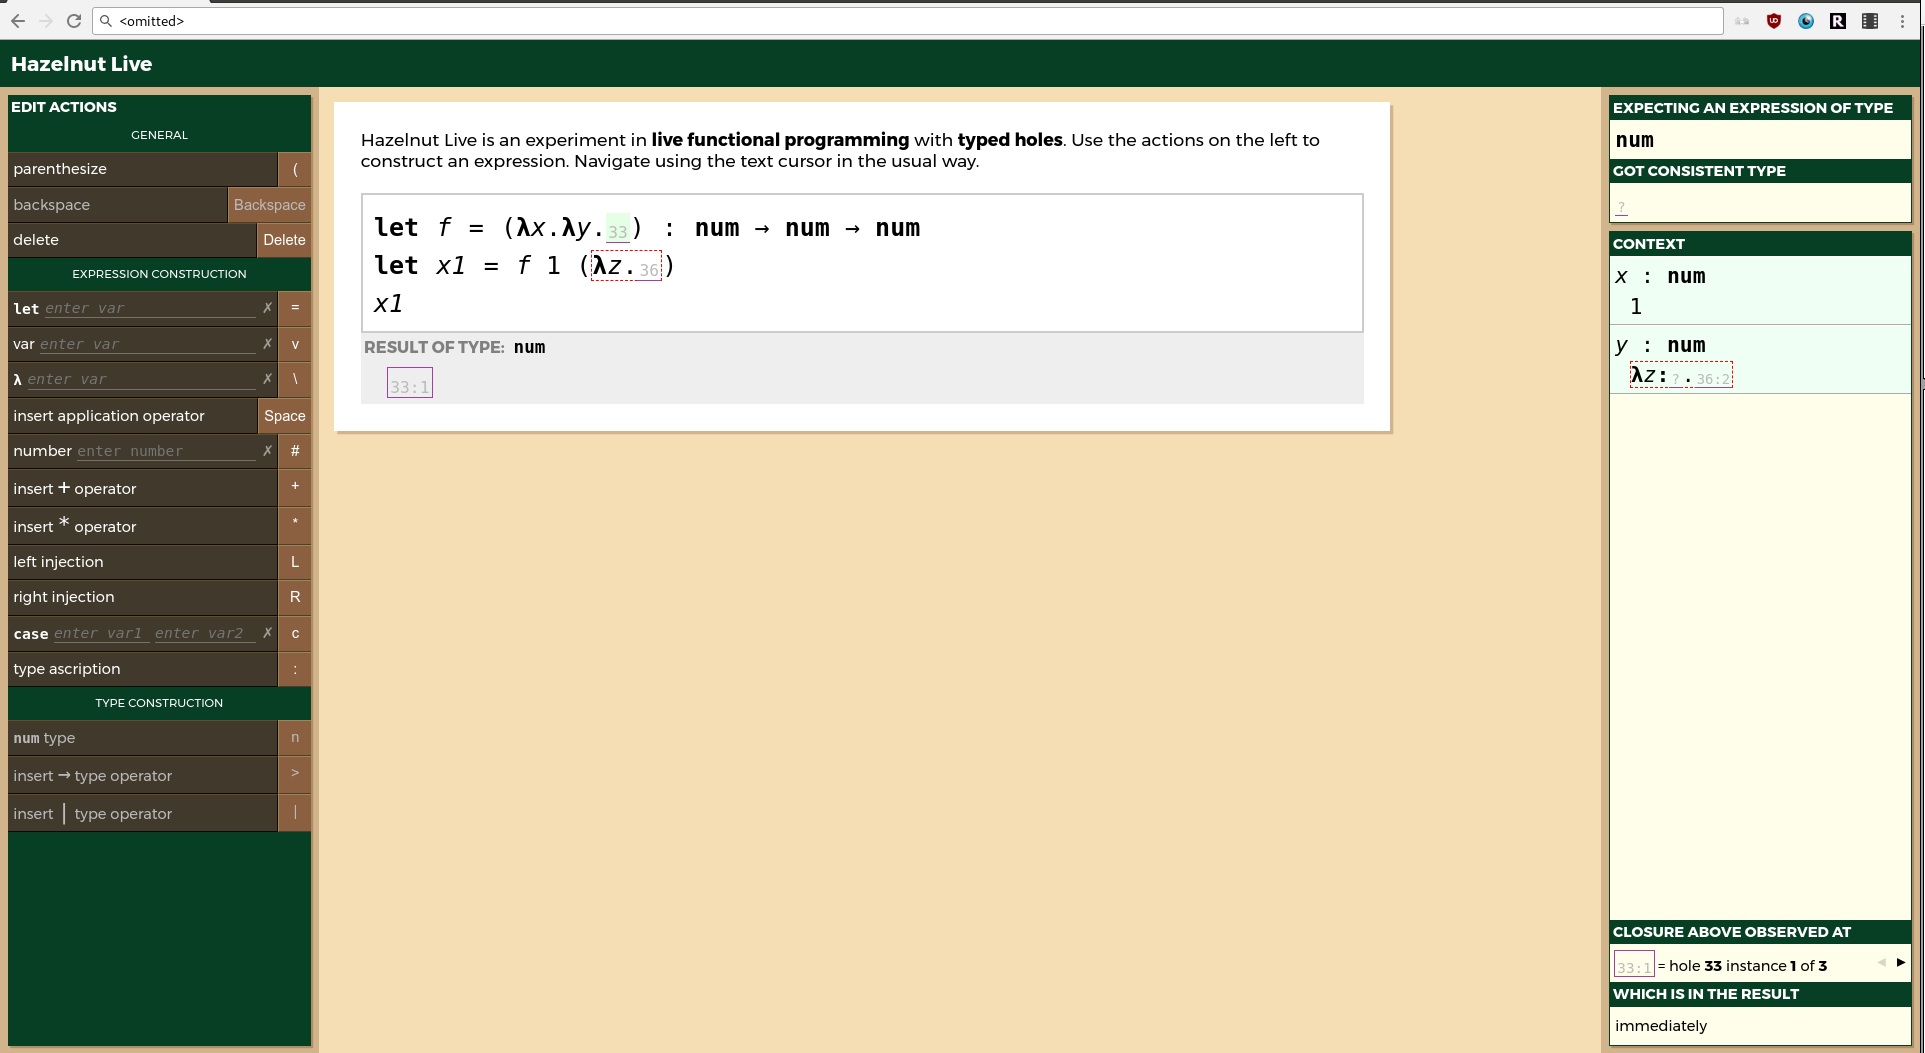
\includegraphics[width=\textwidth]{images/screenshot1.png}
\caption{This screenshot demonstrates both empty and non-empty expression holes as well as the live context inspector.}
\end{figure}

\begin{figure}[h]
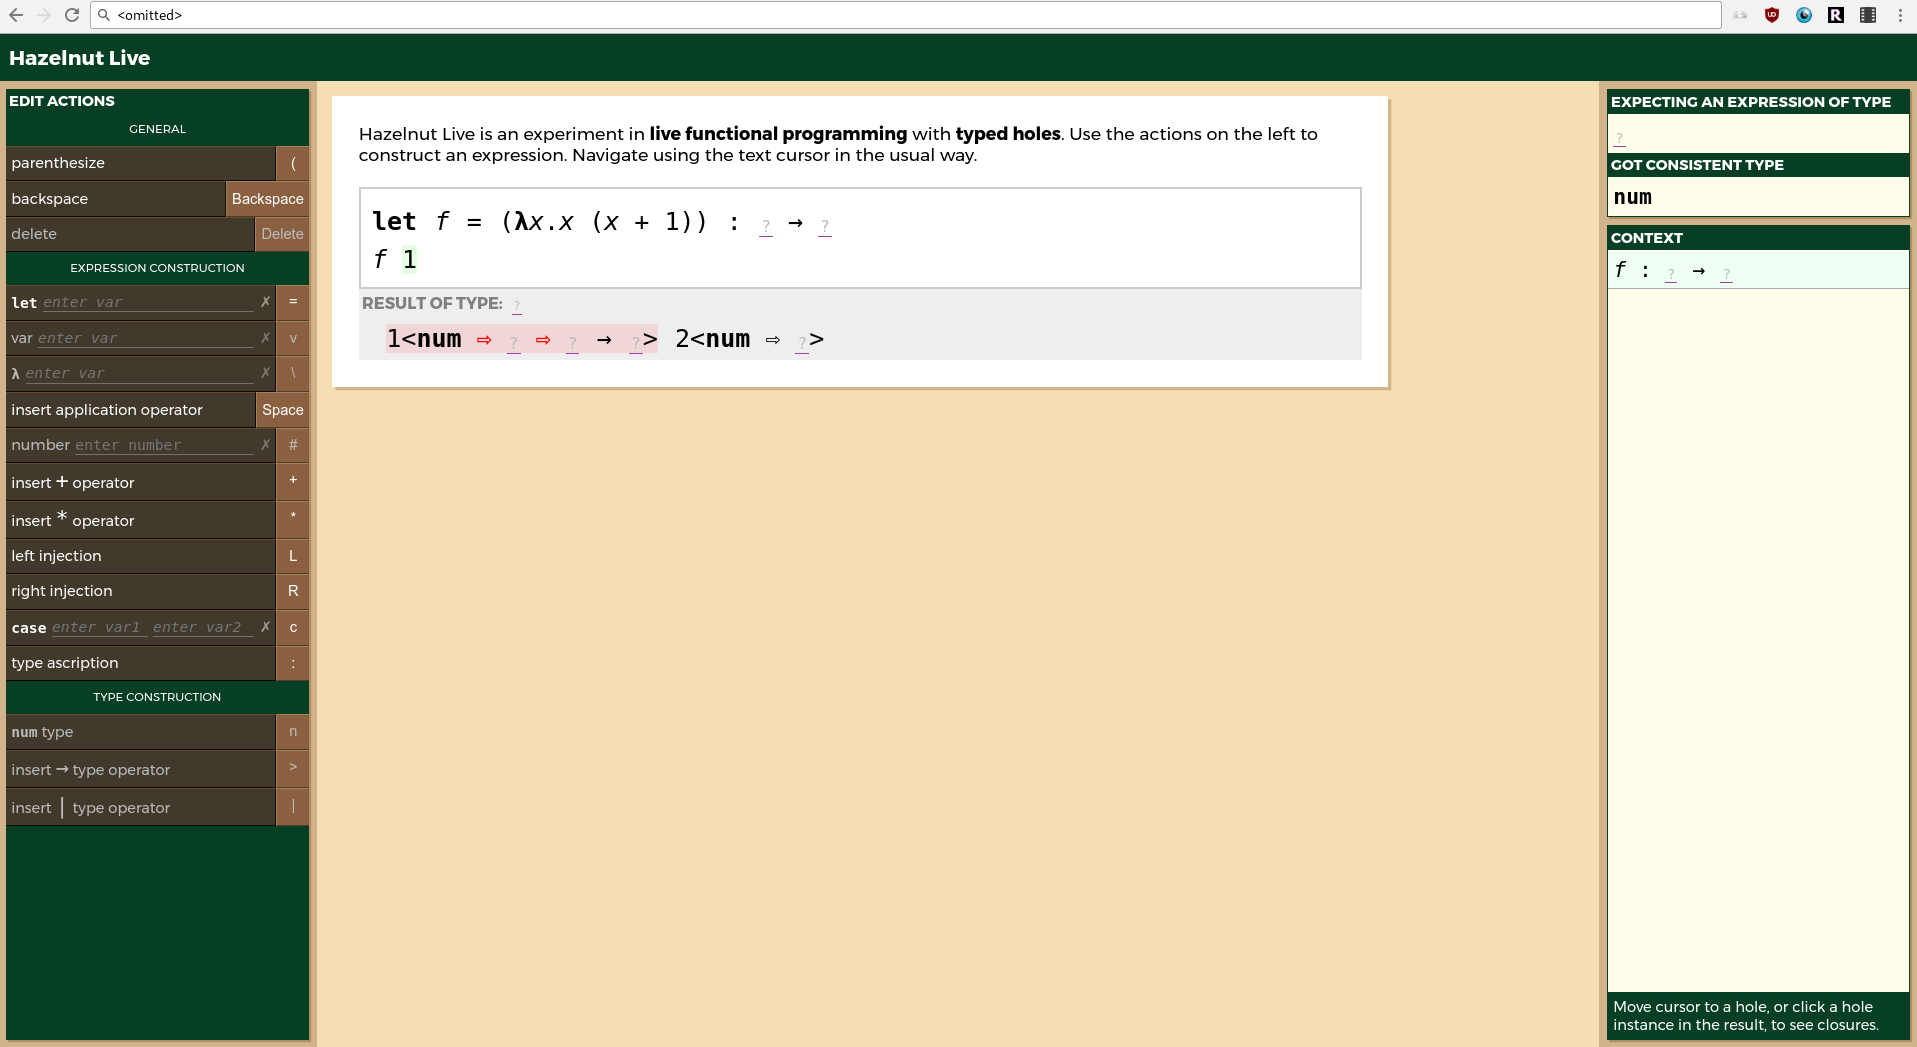
\includegraphics[width=\textwidth]{images/screenshot2.png}
\caption{This screenshot demonstrates dynamic cast failure.}
\end{figure}


\bibliography{references,all.short,hazel_NSF}


\end{document}
